\documentclass{book}
\usepackage[a4paper,top=2.5cm,bottom=2.5cm,left=2.5cm,right=2.5cm]{geometry}
\usepackage{makeidx}
\usepackage{natbib}
\usepackage{graphicx}
\usepackage{multicol}
\usepackage{float}
\usepackage{listings}
\usepackage{color}
\usepackage{ifthen}
\usepackage[table]{xcolor}
\usepackage{textcomp}
\usepackage{alltt}
\usepackage{ifpdf}
\ifpdf
\usepackage[pdftex,
            pagebackref=true,
            colorlinks=true,
            linkcolor=blue,
            unicode
           ]{hyperref}
\else
\usepackage[ps2pdf,
            pagebackref=true,
            colorlinks=true,
            linkcolor=blue,
            unicode
           ]{hyperref}
\usepackage{pspicture}
\fi
\usepackage[utf8]{inputenc}
\usepackage{mathptmx}
\usepackage[scaled=.90]{helvet}
\usepackage{courier}
\usepackage{sectsty}
\usepackage{amssymb}
\usepackage[titles]{tocloft}
\usepackage{doxygen}
\lstset{language=C++,inputencoding=utf8,basicstyle=\footnotesize,breaklines=true,breakatwhitespace=true,tabsize=2,numbers=left }
\makeindex
\setcounter{tocdepth}{3}
\renewcommand{\footrulewidth}{0.4pt}
\renewcommand{\familydefault}{\sfdefault}
\hfuzz=15pt
\setlength{\emergencystretch}{15pt}
\hbadness=750
\tolerance=750
\begin{document}
\hypersetup{pageanchor=false,citecolor=blue}
\begin{titlepage}
\vspace*{7cm}
\begin{center}
{\Large Ventistipes }\\
\vspace*{1cm}
{\large Generated by Doxygen 1.8.3.1}\\
\vspace*{0.5cm}
{\small Thu Mar 14 2013 09:33:27}\\
\end{center}
\end{titlepage}
\clearemptydoublepage
\pagenumbering{roman}
\tableofcontents
\clearemptydoublepage
\pagenumbering{arabic}
\hypersetup{pageanchor=true,citecolor=blue}
\chapter{Data Structure Index}
\section{Data Structures}
Here are the data structures with brief descriptions\-:\begin{DoxyCompactList}
\item\contentsline{section}{\hyperlink{structconnection__struct}{connection\-\_\-struct} }{\pageref{structconnection__struct}}{}
\item\contentsline{section}{\hyperlink{structemail}{email} }{\pageref{structemail}}{}
\item\contentsline{section}{\hyperlink{structpush__info}{push\-\_\-info} }{\pageref{structpush__info}}{}
\item\contentsline{section}{\hyperlink{structquery__struct}{query\-\_\-struct} }{\pageref{structquery__struct}}{}
\end{DoxyCompactList}

\chapter{File Index}
\section{File List}
Here is a list of all files with brief descriptions\-:\begin{DoxyCompactList}
\item\contentsline{section}{include/\hyperlink{email_8h}{email.\-h} }{\pageref{email_8h}}{}
\item\contentsline{section}{include/\hyperlink{macros_8h}{macros.\-h} }{\pageref{macros_8h}}{}
\item\contentsline{section}{include/\hyperlink{postgres_8h}{postgres.\-h} }{\pageref{postgres_8h}}{}
\item\contentsline{section}{include/\hyperlink{safefree_8h}{safefree.\-h} }{\pageref{safefree_8h}}{}
\item\contentsline{section}{include/\hyperlink{smtp_8h}{smtp.\-h} }{\pageref{smtp_8h}}{}
\item\contentsline{section}{include/\hyperlink{string__helpers_8h}{string\-\_\-helpers.\-h} }{\pageref{string__helpers_8h}}{}
\item\contentsline{section}{include/config/\hyperlink{dbinfo_8h}{dbinfo.\-h} }{\pageref{dbinfo_8h}}{}
\item\contentsline{section}{include/config/\hyperlink{gcm__key_8h}{gcm\-\_\-key.\-h} }{\pageref{gcm__key_8h}}{}
\item\contentsline{section}{include/push/\hyperlink{android_8h}{android.\-h} }{\pageref{android_8h}}{}
\item\contentsline{section}{include/push/\hyperlink{push_8h}{push.\-h} }{\pageref{push_8h}}{}
\item\contentsline{section}{src/\hyperlink{email_8c}{email.\-c} }{\pageref{email_8c}}{}
\item\contentsline{section}{src/\hyperlink{main_8c}{main.\-c} }{\pageref{main_8c}}{}
\item\contentsline{section}{src/\hyperlink{postgres_8c}{postgres.\-c} }{\pageref{postgres_8c}}{}
\item\contentsline{section}{src/\hyperlink{safefree_8c}{safefree.\-c} }{\pageref{safefree_8c}}{}
\item\contentsline{section}{src/\hyperlink{smtp_8c}{smtp.\-c} }{\pageref{smtp_8c}}{}
\item\contentsline{section}{src/\hyperlink{string__helpers_8c}{string\-\_\-helpers.\-c} }{\pageref{string__helpers_8c}}{}
\item\contentsline{section}{src/push/\hyperlink{android_8c}{android.\-c} }{\pageref{android_8c}}{}
\item\contentsline{section}{src/push/\hyperlink{push_8c}{push.\-c} }{\pageref{push_8c}}{}
\end{DoxyCompactList}

\chapter{Data Structure Documentation}
\hypertarget{structconnection__struct}{\section{connection\-\_\-struct Struct Reference}
\label{structconnection__struct}\index{connection\-\_\-struct@{connection\-\_\-struct}}
}


Collaboration diagram for connection\-\_\-struct\-:
\nopagebreak
\begin{figure}[H]
\begin{center}
\leavevmode
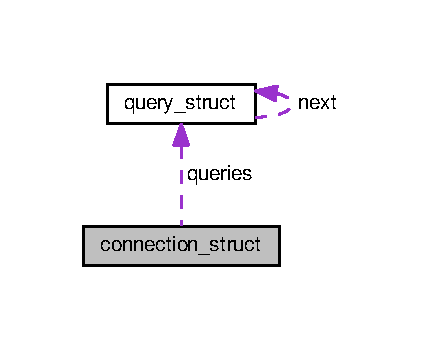
\includegraphics[width=202pt]{structconnection__struct__coll__graph}
\end{center}
\end{figure}
\subsection*{Data Fields}
\begin{DoxyCompactItemize}
\item 
P\-Gconn $\ast$ \hyperlink{structconnection__struct_af4516154f33e07be1eadff88fab71465}{conn}
\item 
struct \hyperlink{structquery__struct}{query\-\_\-struct} $\ast$ \hyperlink{structconnection__struct_ae8bf023f24dae989954803b34f8346f6}{queries}
\item 
unsigned int \hyperlink{structconnection__struct_a9d003902114bc45d2d33eb953579673a}{query\-\_\-count}
\item 
unsigned int \hyperlink{structconnection__struct_a2e4c5444712d727aaeb1050a4c734d4f}{idle\-\_\-ticker}
\end{DoxyCompactItemize}


\subsection{Field Documentation}
\hypertarget{structconnection__struct_af4516154f33e07be1eadff88fab71465}{\index{connection\-\_\-struct@{connection\-\_\-struct}!conn@{conn}}
\index{conn@{conn}!connection_struct@{connection\-\_\-struct}}
\subsubsection[{conn}]{\setlength{\rightskip}{0pt plus 5cm}P\-Gconn$\ast$ conn}}\label{structconnection__struct_af4516154f33e07be1eadff88fab71465}
\hypertarget{structconnection__struct_a2e4c5444712d727aaeb1050a4c734d4f}{\index{connection\-\_\-struct@{connection\-\_\-struct}!idle\-\_\-ticker@{idle\-\_\-ticker}}
\index{idle\-\_\-ticker@{idle\-\_\-ticker}!connection_struct@{connection\-\_\-struct}}
\subsubsection[{idle\-\_\-ticker}]{\setlength{\rightskip}{0pt plus 5cm}unsigned int idle\-\_\-ticker}}\label{structconnection__struct_a2e4c5444712d727aaeb1050a4c734d4f}
\hypertarget{structconnection__struct_ae8bf023f24dae989954803b34f8346f6}{\index{connection\-\_\-struct@{connection\-\_\-struct}!queries@{queries}}
\index{queries@{queries}!connection_struct@{connection\-\_\-struct}}
\subsubsection[{queries}]{\setlength{\rightskip}{0pt plus 5cm}struct {\bf query\-\_\-struct}$\ast$ queries}}\label{structconnection__struct_ae8bf023f24dae989954803b34f8346f6}
\hypertarget{structconnection__struct_a9d003902114bc45d2d33eb953579673a}{\index{connection\-\_\-struct@{connection\-\_\-struct}!query\-\_\-count@{query\-\_\-count}}
\index{query\-\_\-count@{query\-\_\-count}!connection_struct@{connection\-\_\-struct}}
\subsubsection[{query\-\_\-count}]{\setlength{\rightskip}{0pt plus 5cm}unsigned int query\-\_\-count}}\label{structconnection__struct_a9d003902114bc45d2d33eb953579673a}


The documentation for this struct was generated from the following file\-:\begin{DoxyCompactItemize}
\item 
src/\hyperlink{postgres_8c}{postgres.\-c}\end{DoxyCompactItemize}

\hypertarget{structemail}{\section{email Struct Reference}
\label{structemail}\index{email@{email}}
}


{\ttfamily \#include $<$email.\-h$>$}

\subsection*{Data Fields}
\begin{DoxyCompactItemize}
\item 
char \hyperlink{structemail_ab6507ffd67fc6059c2aa721b7b8f8f03}{ehlo}
\item 
char $\ast$ \hyperlink{structemail_a765533dfc643627999c751f7e1514664}{from}
\item 
char $\ast$ \hyperlink{structemail_a501cf38e14279529940ea1df44ca4535}{to} \mbox{[}\hyperlink{email_8h_a14de6dbbf65a1bde6916200bf0215c23}{M\-A\-X\-\_\-\-R\-E\-C\-I\-P\-I\-E\-N\-T\-S}\mbox{]}
\item 
char $\ast$ \hyperlink{structemail_ae31ac864419a577c2982907c23b426d3}{subject}
\item 
char $\ast$ \hyperlink{structemail_a91a70b77df95bd8b0830b49a094c2acb}{data}
\item 
struct bufferevent $\ast$ \hyperlink{structemail_a7a6bf7d3dd8ad7622482a90042e470ef}{bev}
\item 
char \hyperlink{structemail_a000e34997df38c2005a83d63e67d9282}{mode}
\end{DoxyCompactItemize}


\subsection{Field Documentation}
\hypertarget{structemail_a7a6bf7d3dd8ad7622482a90042e470ef}{\index{email@{email}!bev@{bev}}
\index{bev@{bev}!email@{email}}
\subsubsection[{bev}]{\setlength{\rightskip}{0pt plus 5cm}struct bufferevent$\ast$ bev}}\label{structemail_a7a6bf7d3dd8ad7622482a90042e470ef}
\hypertarget{structemail_a91a70b77df95bd8b0830b49a094c2acb}{\index{email@{email}!data@{data}}
\index{data@{data}!email@{email}}
\subsubsection[{data}]{\setlength{\rightskip}{0pt plus 5cm}char$\ast$ data}}\label{structemail_a91a70b77df95bd8b0830b49a094c2acb}
\hypertarget{structemail_ab6507ffd67fc6059c2aa721b7b8f8f03}{\index{email@{email}!ehlo@{ehlo}}
\index{ehlo@{ehlo}!email@{email}}
\subsubsection[{ehlo}]{\setlength{\rightskip}{0pt plus 5cm}char ehlo}}\label{structemail_ab6507ffd67fc6059c2aa721b7b8f8f03}
\hypertarget{structemail_a765533dfc643627999c751f7e1514664}{\index{email@{email}!from@{from}}
\index{from@{from}!email@{email}}
\subsubsection[{from}]{\setlength{\rightskip}{0pt plus 5cm}char$\ast$ from}}\label{structemail_a765533dfc643627999c751f7e1514664}
\hypertarget{structemail_a000e34997df38c2005a83d63e67d9282}{\index{email@{email}!mode@{mode}}
\index{mode@{mode}!email@{email}}
\subsubsection[{mode}]{\setlength{\rightskip}{0pt plus 5cm}char mode}}\label{structemail_a000e34997df38c2005a83d63e67d9282}
\hypertarget{structemail_ae31ac864419a577c2982907c23b426d3}{\index{email@{email}!subject@{subject}}
\index{subject@{subject}!email@{email}}
\subsubsection[{subject}]{\setlength{\rightskip}{0pt plus 5cm}char$\ast$ subject}}\label{structemail_ae31ac864419a577c2982907c23b426d3}
\hypertarget{structemail_a501cf38e14279529940ea1df44ca4535}{\index{email@{email}!to@{to}}
\index{to@{to}!email@{email}}
\subsubsection[{to}]{\setlength{\rightskip}{0pt plus 5cm}char$\ast$ to\mbox{[}{\bf M\-A\-X\-\_\-\-R\-E\-C\-I\-P\-I\-E\-N\-T\-S}\mbox{]}}}\label{structemail_a501cf38e14279529940ea1df44ca4535}


The documentation for this struct was generated from the following file\-:\begin{DoxyCompactItemize}
\item 
include/\hyperlink{email_8h}{email.\-h}\end{DoxyCompactItemize}

\hypertarget{structpush__info}{\section{push\-\_\-info Struct Reference}
\label{structpush__info}\index{push\-\_\-info@{push\-\_\-info}}
}


{\ttfamily \#include $<$push.\-h$>$}

\subsection*{Data Fields}
\begin{DoxyCompactItemize}
\item 
char $\ast$ \hyperlink{structpush__info_ae31ac864419a577c2982907c23b426d3}{subject}
\item 
char $\ast$ \hyperlink{structpush__info_a91a70b77df95bd8b0830b49a094c2acb}{data}
\item 
char $\ast$ \hyperlink{structpush__info_ab092ba1f84e458809eb91a5786b281de}{sender}
\item 
struct event\-\_\-base $\ast$ \hyperlink{structpush__info_ac1c1d71aa37cb71608f4f802bb85b200}{event\-\_\-base}
\end{DoxyCompactItemize}


\subsection{Field Documentation}
\hypertarget{structpush__info_a91a70b77df95bd8b0830b49a094c2acb}{\index{push\-\_\-info@{push\-\_\-info}!data@{data}}
\index{data@{data}!push_info@{push\-\_\-info}}
\subsubsection[{data}]{\setlength{\rightskip}{0pt plus 5cm}char$\ast$ data}}\label{structpush__info_a91a70b77df95bd8b0830b49a094c2acb}
\hypertarget{structpush__info_ac1c1d71aa37cb71608f4f802bb85b200}{\index{push\-\_\-info@{push\-\_\-info}!event\-\_\-base@{event\-\_\-base}}
\index{event\-\_\-base@{event\-\_\-base}!push_info@{push\-\_\-info}}
\subsubsection[{event\-\_\-base}]{\setlength{\rightskip}{0pt plus 5cm}struct event\-\_\-base$\ast$ event\-\_\-base}}\label{structpush__info_ac1c1d71aa37cb71608f4f802bb85b200}
\hypertarget{structpush__info_ab092ba1f84e458809eb91a5786b281de}{\index{push\-\_\-info@{push\-\_\-info}!sender@{sender}}
\index{sender@{sender}!push_info@{push\-\_\-info}}
\subsubsection[{sender}]{\setlength{\rightskip}{0pt plus 5cm}char$\ast$ sender}}\label{structpush__info_ab092ba1f84e458809eb91a5786b281de}
\hypertarget{structpush__info_ae31ac864419a577c2982907c23b426d3}{\index{push\-\_\-info@{push\-\_\-info}!subject@{subject}}
\index{subject@{subject}!push_info@{push\-\_\-info}}
\subsubsection[{subject}]{\setlength{\rightskip}{0pt plus 5cm}char$\ast$ subject}}\label{structpush__info_ae31ac864419a577c2982907c23b426d3}


The documentation for this struct was generated from the following file\-:\begin{DoxyCompactItemize}
\item 
include/push/\hyperlink{push_8h}{push.\-h}\end{DoxyCompactItemize}

\hypertarget{structquery__struct}{\section{query\-\_\-struct Struct Reference}
\label{structquery__struct}\index{query\-\_\-struct@{query\-\_\-struct}}
}


Collaboration diagram for query\-\_\-struct\-:
\nopagebreak
\begin{figure}[H]
\begin{center}
\leavevmode
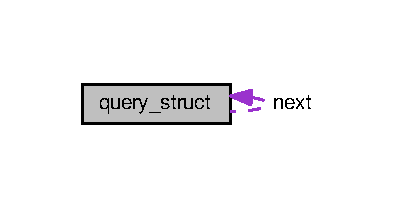
\includegraphics[width=190pt]{structquery__struct__coll__graph}
\end{center}
\end{figure}
\subsection*{Data Fields}
\begin{DoxyCompactItemize}
\item 
void($\ast$ \hyperlink{structquery__struct_a9e358202526ef6f362060add447a5822}{callback} )(P\-Gresult $\ast$, void $\ast$, char $\ast$)
\item 
void $\ast$ \hyperlink{structquery__struct_ae376f130b17d169ee51be68077a89ed0}{context}
\item 
char $\ast$ \hyperlink{structquery__struct_af26982218484ec3fdcb8f7d92e864a9b}{query}
\item 
char \hyperlink{structquery__struct_a59a9dc1eb9f9942b0a09df5acb7a31ff}{sent}
\item 
struct \hyperlink{structquery__struct}{query\-\_\-struct} $\ast$ \hyperlink{structquery__struct_addbda803c3d54ffae5a8c673ea3e701e}{next}
\end{DoxyCompactItemize}


\subsection{Field Documentation}
\hypertarget{structquery__struct_a9e358202526ef6f362060add447a5822}{\index{query\-\_\-struct@{query\-\_\-struct}!callback@{callback}}
\index{callback@{callback}!query_struct@{query\-\_\-struct}}
\subsubsection[{callback}]{\setlength{\rightskip}{0pt plus 5cm}void($\ast$ callback)(P\-Gresult $\ast$, void $\ast$, char $\ast$)}}\label{structquery__struct_a9e358202526ef6f362060add447a5822}
\hypertarget{structquery__struct_ae376f130b17d169ee51be68077a89ed0}{\index{query\-\_\-struct@{query\-\_\-struct}!context@{context}}
\index{context@{context}!query_struct@{query\-\_\-struct}}
\subsubsection[{context}]{\setlength{\rightskip}{0pt plus 5cm}void$\ast$ context}}\label{structquery__struct_ae376f130b17d169ee51be68077a89ed0}
\hypertarget{structquery__struct_addbda803c3d54ffae5a8c673ea3e701e}{\index{query\-\_\-struct@{query\-\_\-struct}!next@{next}}
\index{next@{next}!query_struct@{query\-\_\-struct}}
\subsubsection[{next}]{\setlength{\rightskip}{0pt plus 5cm}struct {\bf query\-\_\-struct}$\ast$ next}}\label{structquery__struct_addbda803c3d54ffae5a8c673ea3e701e}
\hypertarget{structquery__struct_af26982218484ec3fdcb8f7d92e864a9b}{\index{query\-\_\-struct@{query\-\_\-struct}!query@{query}}
\index{query@{query}!query_struct@{query\-\_\-struct}}
\subsubsection[{query}]{\setlength{\rightskip}{0pt plus 5cm}char$\ast$ query}}\label{structquery__struct_af26982218484ec3fdcb8f7d92e864a9b}
\hypertarget{structquery__struct_a59a9dc1eb9f9942b0a09df5acb7a31ff}{\index{query\-\_\-struct@{query\-\_\-struct}!sent@{sent}}
\index{sent@{sent}!query_struct@{query\-\_\-struct}}
\subsubsection[{sent}]{\setlength{\rightskip}{0pt plus 5cm}char sent}}\label{structquery__struct_a59a9dc1eb9f9942b0a09df5acb7a31ff}


The documentation for this struct was generated from the following file\-:\begin{DoxyCompactItemize}
\item 
src/\hyperlink{postgres_8c}{postgres.\-c}\end{DoxyCompactItemize}

\chapter{File Documentation}
\hypertarget{dbinfo_8h}{\section{include/config/dbinfo.h File Reference}
\label{dbinfo_8h}\index{include/config/dbinfo.\-h@{include/config/dbinfo.\-h}}
}
This graph shows which files directly or indirectly include this file\-:
\nopagebreak
\begin{figure}[H]
\begin{center}
\leavevmode
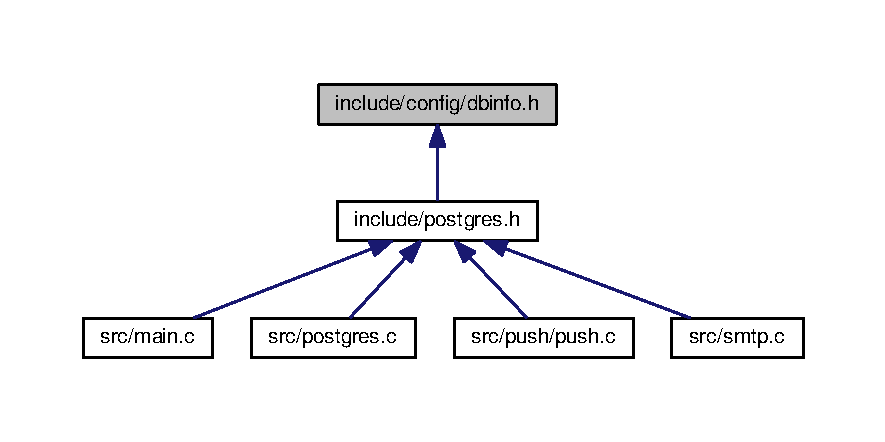
\includegraphics[width=350pt]{dbinfo_8h__dep__incl}
\end{center}
\end{figure}

\hypertarget{gcm__key_8h}{\section{include/config/gcm\-\_\-key.h File Reference}
\label{gcm__key_8h}\index{include/config/gcm\-\_\-key.\-h@{include/config/gcm\-\_\-key.\-h}}
}
This graph shows which files directly or indirectly include this file\-:
\nopagebreak
\begin{figure}[H]
\begin{center}
\leavevmode
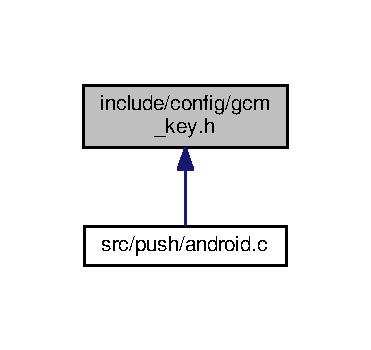
\includegraphics[width=178pt]{gcm__key_8h__dep__incl}
\end{center}
\end{figure}

\hypertarget{email_8h}{\section{include/email.h File Reference}
\label{email_8h}\index{include/email.\-h@{include/email.\-h}}
}
This graph shows which files directly or indirectly include this file\-:
\nopagebreak
\begin{figure}[H]
\begin{center}
\leavevmode
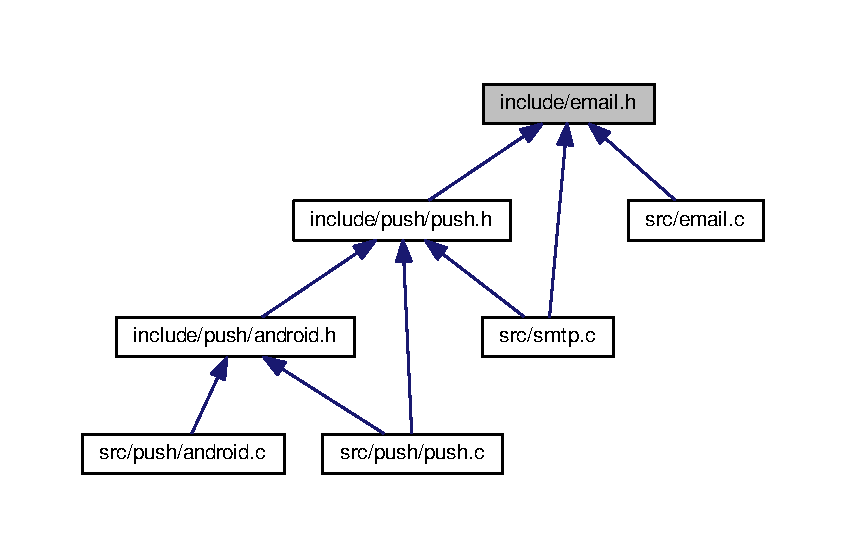
\includegraphics[width=350pt]{email_8h__dep__incl}
\end{center}
\end{figure}
\subsection*{Data Structures}
\begin{DoxyCompactItemize}
\item 
struct \hyperlink{structemail}{email}
\end{DoxyCompactItemize}
\subsection*{Macros}
\begin{DoxyCompactItemize}
\item 
\#define \hyperlink{email_8h_a14de6dbbf65a1bde6916200bf0215c23}{M\-A\-X\-\_\-\-R\-E\-C\-I\-P\-I\-E\-N\-T\-S}~100
\end{DoxyCompactItemize}
\subsection*{Functions}
\begin{DoxyCompactItemize}
\item 
struct \hyperlink{structemail}{email} $\ast$ \hyperlink{email_8h_a92d36df971c6ea4b807f191461774628}{new\-\_\-email} ()
\item 
void \hyperlink{email_8h_a5227fadfd1014417c4ce6bfc4a925592}{delete\-\_\-email} (struct \hyperlink{structemail}{email} $\ast$\hyperlink{structemail}{email})
\item 
int \hyperlink{email_8h_a21caf89afa30b60df1eec81bfb48e6d0}{email\-\_\-set\-\_\-sender} (struct \hyperlink{structemail}{email} $\ast$\hyperlink{structemail}{email}, char $\ast$from)
\item 
int \hyperlink{email_8h_a634d99bdaba585890305ea9f86312c09}{email\-\_\-add\-\_\-recipient} (struct \hyperlink{structemail}{email} $\ast$\hyperlink{structemail}{email}, char $\ast$to)
\item 
int \hyperlink{email_8h_a46ed54490f60eccc2513cae45ef8adfb}{email\-\_\-has\-\_\-recipients} (struct \hyperlink{structemail}{email} $\ast$\hyperlink{structemail}{email})
\item 
char $\ast$ \hyperlink{email_8h_a8b8b8be04443bcbad35d3100929e2a8f}{email\-\_\-get\-\_\-last\-\_\-recipient} (struct \hyperlink{structemail}{email} $\ast$\hyperlink{structemail}{email})
\item 
int \hyperlink{email_8h_acf2b3d9d17180be215d06b5267bb5042}{email\-\_\-remove\-\_\-email\-\_\-from\-\_\-recipients} (struct \hyperlink{structemail}{email} $\ast$\hyperlink{structemail}{email}, char $\ast$addr)
\item 
int \hyperlink{email_8h_a164bbbf7611e6a4f842a9d9699d756a1}{email\-\_\-set\-\_\-subject} (struct \hyperlink{structemail}{email} $\ast$\hyperlink{structemail}{email}, char $\ast$line)
\item 
void \hyperlink{email_8h_a39795abc038b09b975b2dfaee3067dae}{email\-\_\-for\-\_\-each\-\_\-recipient} (struct \hyperlink{structemail}{email} $\ast$\hyperlink{structemail}{email}, void $\ast$context, void($\ast$execute)(char $\ast$address, void $\ast$context, struct \hyperlink{structemail}{email} $\ast$\hyperlink{structemail}{email}))
\item 
int \hyperlink{email_8h_a179442b2783a7258bfa8e5f69e758a58}{email\-\_\-append\-\_\-data} (struct \hyperlink{structemail}{email} $\ast$\hyperlink{structemail}{email}, char $\ast$data)
\end{DoxyCompactItemize}


\subsection{Macro Definition Documentation}
\hypertarget{email_8h_a14de6dbbf65a1bde6916200bf0215c23}{\index{email.\-h@{email.\-h}!M\-A\-X\-\_\-\-R\-E\-C\-I\-P\-I\-E\-N\-T\-S@{M\-A\-X\-\_\-\-R\-E\-C\-I\-P\-I\-E\-N\-T\-S}}
\index{M\-A\-X\-\_\-\-R\-E\-C\-I\-P\-I\-E\-N\-T\-S@{M\-A\-X\-\_\-\-R\-E\-C\-I\-P\-I\-E\-N\-T\-S}!email.h@{email.\-h}}
\subsubsection[{M\-A\-X\-\_\-\-R\-E\-C\-I\-P\-I\-E\-N\-T\-S}]{\setlength{\rightskip}{0pt plus 5cm}\#define M\-A\-X\-\_\-\-R\-E\-C\-I\-P\-I\-E\-N\-T\-S~100}}\label{email_8h_a14de6dbbf65a1bde6916200bf0215c23}


\subsection{Function Documentation}
\hypertarget{email_8h_a5227fadfd1014417c4ce6bfc4a925592}{\index{email.\-h@{email.\-h}!delete\-\_\-email@{delete\-\_\-email}}
\index{delete\-\_\-email@{delete\-\_\-email}!email.h@{email.\-h}}
\subsubsection[{delete\-\_\-email}]{\setlength{\rightskip}{0pt plus 5cm}void delete\-\_\-email (
\begin{DoxyParamCaption}
\item[{struct {\bf email} $\ast$}]{email}
\end{DoxyParamCaption}
)}}\label{email_8h_a5227fadfd1014417c4ce6bfc4a925592}
Clean up this email structure 
\begin{DoxyParams}{Parameters}
{\em email} & The email structure we want to clean up \\
\hline
\end{DoxyParams}
\hypertarget{email_8h_a634d99bdaba585890305ea9f86312c09}{\index{email.\-h@{email.\-h}!email\-\_\-add\-\_\-recipient@{email\-\_\-add\-\_\-recipient}}
\index{email\-\_\-add\-\_\-recipient@{email\-\_\-add\-\_\-recipient}!email.h@{email.\-h}}
\subsubsection[{email\-\_\-add\-\_\-recipient}]{\setlength{\rightskip}{0pt plus 5cm}int email\-\_\-add\-\_\-recipient (
\begin{DoxyParamCaption}
\item[{struct {\bf email} $\ast$}]{email, }
\item[{char $\ast$}]{to}
\end{DoxyParamCaption}
)}}\label{email_8h_a634d99bdaba585890305ea9f86312c09}
Add a recipient to our email structure 
\begin{DoxyParams}{Parameters}
{\em email} & The email structure we want to have this recipient \\
\hline
{\em to} & The recipient's email address \\
\hline
\end{DoxyParams}
\begin{DoxyReturn}{Returns}
1 if added correctly, 0 if not added this will only occur when there are more than M\-A\-X\-\_\-\-R\-E\-C\-I\-P\-I\-E\-N\-T\-S recipients or if the email isn't valid 
\end{DoxyReturn}
\hypertarget{email_8h_a179442b2783a7258bfa8e5f69e758a58}{\index{email.\-h@{email.\-h}!email\-\_\-append\-\_\-data@{email\-\_\-append\-\_\-data}}
\index{email\-\_\-append\-\_\-data@{email\-\_\-append\-\_\-data}!email.h@{email.\-h}}
\subsubsection[{email\-\_\-append\-\_\-data}]{\setlength{\rightskip}{0pt plus 5cm}int email\-\_\-append\-\_\-data (
\begin{DoxyParamCaption}
\item[{struct {\bf email} $\ast$}]{email, }
\item[{char $\ast$}]{data}
\end{DoxyParamCaption}
)}}\label{email_8h_a179442b2783a7258bfa8e5f69e758a58}
Parse a raw line to 'append' it to the data field in email 
\begin{DoxyParams}{Parameters}
{\em email} & The email structure we want to have this data \\
\hline
{\em data} & The data we want to append \\
\hline
\end{DoxyParams}
\begin{DoxyReturn}{Returns}
1 in case we're in the right mode, else it'll return 0 
\end{DoxyReturn}
\hypertarget{email_8h_a39795abc038b09b975b2dfaee3067dae}{\index{email.\-h@{email.\-h}!email\-\_\-for\-\_\-each\-\_\-recipient@{email\-\_\-for\-\_\-each\-\_\-recipient}}
\index{email\-\_\-for\-\_\-each\-\_\-recipient@{email\-\_\-for\-\_\-each\-\_\-recipient}!email.h@{email.\-h}}
\subsubsection[{email\-\_\-for\-\_\-each\-\_\-recipient}]{\setlength{\rightskip}{0pt plus 5cm}void email\-\_\-for\-\_\-each\-\_\-recipient (
\begin{DoxyParamCaption}
\item[{struct {\bf email} $\ast$}]{email, }
\item[{void $\ast$}]{context, }
\item[{void($\ast$)(char $\ast$address, void $\ast$context, struct {\bf email} $\ast${\bf email})}]{execute}
\end{DoxyParamCaption}
)}}\label{email_8h_a39795abc038b09b975b2dfaee3067dae}
Execute this function pointer for each recipient 
\begin{DoxyParams}{Parameters}
{\em email} & The email structure to use for the recipients \\
\hline
{\em context} & Void pointer to pass to the function pointer \\
\hline
{\em execute} & The function pointer to execute for each recipient \\
\hline
\end{DoxyParams}
\hypertarget{email_8h_a8b8b8be04443bcbad35d3100929e2a8f}{\index{email.\-h@{email.\-h}!email\-\_\-get\-\_\-last\-\_\-recipient@{email\-\_\-get\-\_\-last\-\_\-recipient}}
\index{email\-\_\-get\-\_\-last\-\_\-recipient@{email\-\_\-get\-\_\-last\-\_\-recipient}!email.h@{email.\-h}}
\subsubsection[{email\-\_\-get\-\_\-last\-\_\-recipient}]{\setlength{\rightskip}{0pt plus 5cm}char$\ast$ email\-\_\-get\-\_\-last\-\_\-recipient (
\begin{DoxyParamCaption}
\item[{struct {\bf email} $\ast$}]{email}
\end{DoxyParamCaption}
)}}\label{email_8h_a8b8b8be04443bcbad35d3100929e2a8f}
Get the last recipient \begin{DoxyReturn}{Returns}
Returns the last recipient in the to array returns N\-U\-L\-L if there are no recipients 
\end{DoxyReturn}
\hypertarget{email_8h_a46ed54490f60eccc2513cae45ef8adfb}{\index{email.\-h@{email.\-h}!email\-\_\-has\-\_\-recipients@{email\-\_\-has\-\_\-recipients}}
\index{email\-\_\-has\-\_\-recipients@{email\-\_\-has\-\_\-recipients}!email.h@{email.\-h}}
\subsubsection[{email\-\_\-has\-\_\-recipients}]{\setlength{\rightskip}{0pt plus 5cm}int email\-\_\-has\-\_\-recipients (
\begin{DoxyParamCaption}
\item[{struct {\bf email} $\ast$}]{email}
\end{DoxyParamCaption}
)}}\label{email_8h_a46ed54490f60eccc2513cae45ef8adfb}
Simple check if the email structure has the from and to field filled in. 
\begin{DoxyParams}{Parameters}
{\em email} & The email structure we want to check for recipients \\
\hline
\end{DoxyParams}
\begin{DoxyReturn}{Returns}
If it has both the from and at least one recipient it'll return 1, else it'll return 0 
\end{DoxyReturn}
\hypertarget{email_8h_acf2b3d9d17180be215d06b5267bb5042}{\index{email.\-h@{email.\-h}!email\-\_\-remove\-\_\-email\-\_\-from\-\_\-recipients@{email\-\_\-remove\-\_\-email\-\_\-from\-\_\-recipients}}
\index{email\-\_\-remove\-\_\-email\-\_\-from\-\_\-recipients@{email\-\_\-remove\-\_\-email\-\_\-from\-\_\-recipients}!email.h@{email.\-h}}
\subsubsection[{email\-\_\-remove\-\_\-email\-\_\-from\-\_\-recipients}]{\setlength{\rightskip}{0pt plus 5cm}int email\-\_\-remove\-\_\-email\-\_\-from\-\_\-recipients (
\begin{DoxyParamCaption}
\item[{struct {\bf email} $\ast$}]{email, }
\item[{char $\ast$}]{addr}
\end{DoxyParamCaption}
)}}\label{email_8h_acf2b3d9d17180be215d06b5267bb5042}
Remove an email address from the mail structure 
\begin{DoxyParams}{Parameters}
{\em email} & The structure to remove an address from \\
\hline
{\em addr} & T\-He address to remove \\
\hline
\end{DoxyParams}
\begin{DoxyReturn}{Returns}
1 in case there was something deleted, else it'll return 0 
\end{DoxyReturn}
\hypertarget{email_8h_a21caf89afa30b60df1eec81bfb48e6d0}{\index{email.\-h@{email.\-h}!email\-\_\-set\-\_\-sender@{email\-\_\-set\-\_\-sender}}
\index{email\-\_\-set\-\_\-sender@{email\-\_\-set\-\_\-sender}!email.h@{email.\-h}}
\subsubsection[{email\-\_\-set\-\_\-sender}]{\setlength{\rightskip}{0pt plus 5cm}int email\-\_\-set\-\_\-sender (
\begin{DoxyParamCaption}
\item[{struct {\bf email} $\ast$}]{email, }
\item[{char $\ast$}]{from}
\end{DoxyParamCaption}
)}}\label{email_8h_a21caf89afa30b60df1eec81bfb48e6d0}
Set our sender 
\begin{DoxyParams}{Parameters}
{\em email} & The email structure we want to have this sender \\
\hline
{\em from} & The sender's email address \\
\hline
\end{DoxyParams}
\begin{DoxyReturn}{Returns}
1 in case we set it correctly, else we'll return 0 
\end{DoxyReturn}
\hypertarget{email_8h_a164bbbf7611e6a4f842a9d9699d756a1}{\index{email.\-h@{email.\-h}!email\-\_\-set\-\_\-subject@{email\-\_\-set\-\_\-subject}}
\index{email\-\_\-set\-\_\-subject@{email\-\_\-set\-\_\-subject}!email.h@{email.\-h}}
\subsubsection[{email\-\_\-set\-\_\-subject}]{\setlength{\rightskip}{0pt plus 5cm}int email\-\_\-set\-\_\-subject (
\begin{DoxyParamCaption}
\item[{struct {\bf email} $\ast$}]{email, }
\item[{char $\ast$}]{line}
\end{DoxyParamCaption}
)}}\label{email_8h_a164bbbf7611e6a4f842a9d9699d756a1}
Parse the subject and set it to the email structure 
\begin{DoxyParams}{Parameters}
{\em email} & The email structure we want to have the subject \\
\hline
{\em line} & The raw smtp line to parse for the subject \\
\hline
\end{DoxyParams}
\begin{DoxyReturn}{Returns}
1 in case there is a subject set, else it'll return 0 
\end{DoxyReturn}
\hypertarget{email_8h_a92d36df971c6ea4b807f191461774628}{\index{email.\-h@{email.\-h}!new\-\_\-email@{new\-\_\-email}}
\index{new\-\_\-email@{new\-\_\-email}!email.h@{email.\-h}}
\subsubsection[{new\-\_\-email}]{\setlength{\rightskip}{0pt plus 5cm}struct {\bf email}$\ast$ new\-\_\-email (
\begin{DoxyParamCaption}
{}
\end{DoxyParamCaption}
)\hspace{0.3cm}{\ttfamily [read]}}}\label{email_8h_a92d36df971c6ea4b807f191461774628}
Create a new email structure and return this \begin{DoxyReturn}{Returns}
a new email structure 
\end{DoxyReturn}

\hypertarget{macros_8h}{\section{include/macros.h File Reference}
\label{macros_8h}\index{include/macros.\-h@{include/macros.\-h}}
}
{\ttfamily \#include $<$fcntl.\-h$>$}\\*
Include dependency graph for macros.\-h\-:
\nopagebreak
\begin{figure}[H]
\begin{center}
\leavevmode
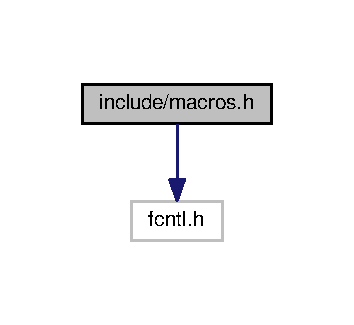
\includegraphics[width=170pt]{macros_8h__incl}
\end{center}
\end{figure}
This graph shows which files directly or indirectly include this file\-:
\nopagebreak
\begin{figure}[H]
\begin{center}
\leavevmode
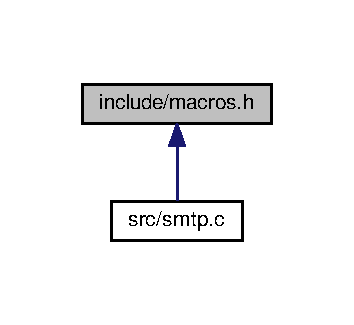
\includegraphics[width=170pt]{macros_8h__dep__incl}
\end{center}
\end{figure}
\subsection*{Macros}
\begin{DoxyCompactItemize}
\item 
\#define \hyperlink{macros_8h_a38f908279b9458412e59e60a421c6f89}{S\-E\-T\-\_\-\-N\-O\-N\-B\-L\-O\-C\-K\-I\-N\-G}(fd)~fcntl(fd, F\-\_\-\-S\-E\-T\-F\-L, fcntl(fd, F\-\_\-\-G\-E\-T\-F\-L) $|$ O\-\_\-\-N\-O\-N\-B\-L\-O\-C\-K)
\end{DoxyCompactItemize}


\subsection{Macro Definition Documentation}
\hypertarget{macros_8h_a38f908279b9458412e59e60a421c6f89}{\index{macros.\-h@{macros.\-h}!S\-E\-T\-\_\-\-N\-O\-N\-B\-L\-O\-C\-K\-I\-N\-G@{S\-E\-T\-\_\-\-N\-O\-N\-B\-L\-O\-C\-K\-I\-N\-G}}
\index{S\-E\-T\-\_\-\-N\-O\-N\-B\-L\-O\-C\-K\-I\-N\-G@{S\-E\-T\-\_\-\-N\-O\-N\-B\-L\-O\-C\-K\-I\-N\-G}!macros.h@{macros.\-h}}
\subsubsection[{S\-E\-T\-\_\-\-N\-O\-N\-B\-L\-O\-C\-K\-I\-N\-G}]{\setlength{\rightskip}{0pt plus 5cm}\#define S\-E\-T\-\_\-\-N\-O\-N\-B\-L\-O\-C\-K\-I\-N\-G(
\begin{DoxyParamCaption}
\item[{}]{fd}
\end{DoxyParamCaption}
)~fcntl(fd, F\-\_\-\-S\-E\-T\-F\-L, fcntl(fd, F\-\_\-\-G\-E\-T\-F\-L) $|$ O\-\_\-\-N\-O\-N\-B\-L\-O\-C\-K)}}\label{macros_8h_a38f908279b9458412e59e60a421c6f89}

\hypertarget{postgres_8h}{\section{include/postgres.h File Reference}
\label{postgres_8h}\index{include/postgres.\-h@{include/postgres.\-h}}
}
{\ttfamily \#include \char`\"{}config/dbinfo.\-h\char`\"{}}\\*
{\ttfamily \#include $<$event2/event.\-h$>$}\\*
{\ttfamily \#include $<$libpq-\/fe.\-h$>$}\\*
Include dependency graph for postgres.\-h\-:
\nopagebreak
\begin{figure}[H]
\begin{center}
\leavevmode
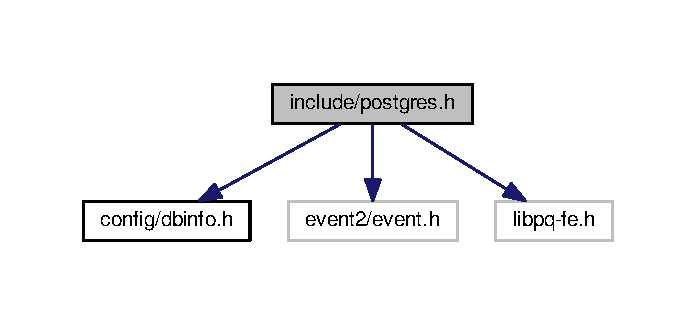
\includegraphics[width=334pt]{postgres_8h__incl}
\end{center}
\end{figure}
This graph shows which files directly or indirectly include this file\-:
\nopagebreak
\begin{figure}[H]
\begin{center}
\leavevmode
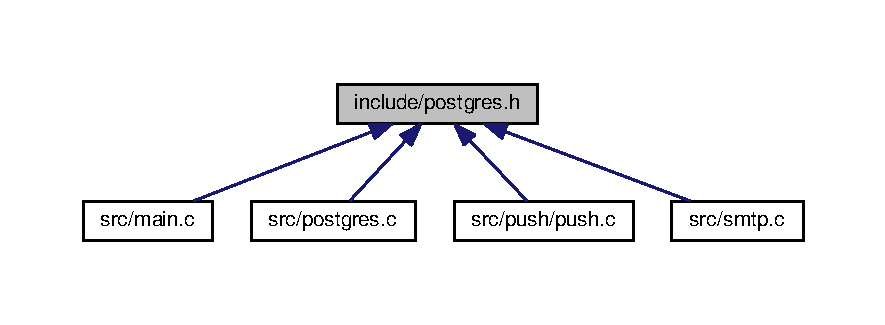
\includegraphics[width=350pt]{postgres_8h__dep__incl}
\end{center}
\end{figure}
\subsection*{Macros}
\begin{DoxyCompactItemize}
\item 
\#define \hyperlink{postgres_8h_a053b7859476cc9867ec62c49e68d3fa1}{M\-A\-X\-\_\-\-C\-O\-N\-N\-E\-C\-T\-I\-O\-N\-S}~10
\item 
\#define \hyperlink{postgres_8h_ac907f69ffe5bba53db033dfbfea600c5}{M\-A\-X\-\_\-\-I\-D\-L\-E\-\_\-\-T\-I\-C\-K\-S}~120
\end{DoxyCompactItemize}
\subsection*{Functions}
\begin{DoxyCompactItemize}
\item 
void \hyperlink{postgres_8h_ad2d8d5718324b20d939a4b04cd3131ff}{init\-Database\-Pool} (struct event\-\_\-base $\ast$base)
\item 
int \hyperlink{postgres_8h_a953a5303803fe3ab05decb3c4c7db8a8}{database\-Query} (char $\ast$query, void($\ast$callback)(P\-Gresult $\ast$, void $\ast$, char $\ast$), void $\ast$context)
\end{DoxyCompactItemize}


\subsection{Macro Definition Documentation}
\hypertarget{postgres_8h_a053b7859476cc9867ec62c49e68d3fa1}{\index{postgres.\-h@{postgres.\-h}!M\-A\-X\-\_\-\-C\-O\-N\-N\-E\-C\-T\-I\-O\-N\-S@{M\-A\-X\-\_\-\-C\-O\-N\-N\-E\-C\-T\-I\-O\-N\-S}}
\index{M\-A\-X\-\_\-\-C\-O\-N\-N\-E\-C\-T\-I\-O\-N\-S@{M\-A\-X\-\_\-\-C\-O\-N\-N\-E\-C\-T\-I\-O\-N\-S}!postgres.h@{postgres.\-h}}
\subsubsection[{M\-A\-X\-\_\-\-C\-O\-N\-N\-E\-C\-T\-I\-O\-N\-S}]{\setlength{\rightskip}{0pt plus 5cm}\#define M\-A\-X\-\_\-\-C\-O\-N\-N\-E\-C\-T\-I\-O\-N\-S~10}}\label{postgres_8h_a053b7859476cc9867ec62c49e68d3fa1}
\hypertarget{postgres_8h_ac907f69ffe5bba53db033dfbfea600c5}{\index{postgres.\-h@{postgres.\-h}!M\-A\-X\-\_\-\-I\-D\-L\-E\-\_\-\-T\-I\-C\-K\-S@{M\-A\-X\-\_\-\-I\-D\-L\-E\-\_\-\-T\-I\-C\-K\-S}}
\index{M\-A\-X\-\_\-\-I\-D\-L\-E\-\_\-\-T\-I\-C\-K\-S@{M\-A\-X\-\_\-\-I\-D\-L\-E\-\_\-\-T\-I\-C\-K\-S}!postgres.h@{postgres.\-h}}
\subsubsection[{M\-A\-X\-\_\-\-I\-D\-L\-E\-\_\-\-T\-I\-C\-K\-S}]{\setlength{\rightskip}{0pt plus 5cm}\#define M\-A\-X\-\_\-\-I\-D\-L\-E\-\_\-\-T\-I\-C\-K\-S~120}}\label{postgres_8h_ac907f69ffe5bba53db033dfbfea600c5}


\subsection{Function Documentation}
\hypertarget{postgres_8h_a953a5303803fe3ab05decb3c4c7db8a8}{\index{postgres.\-h@{postgres.\-h}!database\-Query@{database\-Query}}
\index{database\-Query@{database\-Query}!postgres.h@{postgres.\-h}}
\subsubsection[{database\-Query}]{\setlength{\rightskip}{0pt plus 5cm}int database\-Query (
\begin{DoxyParamCaption}
\item[{char $\ast$}]{query, }
\item[{void($\ast$)(P\-Gresult $\ast$, void $\ast$, char $\ast$)}]{callback, }
\item[{void $\ast$}]{context}
\end{DoxyParamCaption}
)}}\label{postgres_8h_a953a5303803fe3ab05decb3c4c7db8a8}
\hypertarget{postgres_8h_ad2d8d5718324b20d939a4b04cd3131ff}{\index{postgres.\-h@{postgres.\-h}!init\-Database\-Pool@{init\-Database\-Pool}}
\index{init\-Database\-Pool@{init\-Database\-Pool}!postgres.h@{postgres.\-h}}
\subsubsection[{init\-Database\-Pool}]{\setlength{\rightskip}{0pt plus 5cm}void init\-Database\-Pool (
\begin{DoxyParamCaption}
\item[{struct event\-\_\-base $\ast$}]{base}
\end{DoxyParamCaption}
)}}\label{postgres_8h_ad2d8d5718324b20d939a4b04cd3131ff}

\hypertarget{android_8h}{\section{include/push/android.h File Reference}
\label{android_8h}\index{include/push/android.\-h@{include/push/android.\-h}}
}
{\ttfamily \#include \char`\"{}push.\-h\char`\"{}}\\*
{\ttfamily \#include $<$event2/event.\-h$>$}\\*
Include dependency graph for android.\-h\-:
\nopagebreak
\begin{figure}[H]
\begin{center}
\leavevmode
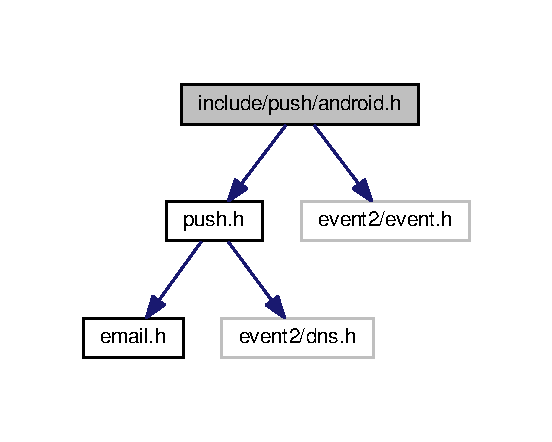
\includegraphics[width=265pt]{android_8h__incl}
\end{center}
\end{figure}
This graph shows which files directly or indirectly include this file\-:
\nopagebreak
\begin{figure}[H]
\begin{center}
\leavevmode
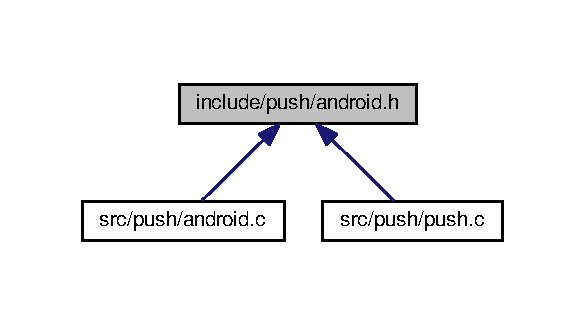
\includegraphics[width=281pt]{android_8h__dep__incl}
\end{center}
\end{figure}
\subsection*{Functions}
\begin{DoxyCompactItemize}
\item 
void \hyperlink{android_8h_a9057dbf56736a0461560bdca4d0eba4c}{android\-\_\-push} (struct \hyperlink{structpush__info}{push\-\_\-info} $\ast$\hyperlink{structpush__info}{push\-\_\-info}, char $\ast$push\-\_\-id, struct \hyperlink{main_8c_ac1c1d71aa37cb71608f4f802bb85b200}{event\-\_\-base} $\ast$\hyperlink{main_8c_ac1c1d71aa37cb71608f4f802bb85b200}{event\-\_\-base})
\end{DoxyCompactItemize}


\subsection{Function Documentation}
\hypertarget{android_8h_a9057dbf56736a0461560bdca4d0eba4c}{\index{android.\-h@{android.\-h}!android\-\_\-push@{android\-\_\-push}}
\index{android\-\_\-push@{android\-\_\-push}!android.h@{android.\-h}}
\subsubsection[{android\-\_\-push}]{\setlength{\rightskip}{0pt plus 5cm}void android\-\_\-push (
\begin{DoxyParamCaption}
\item[{struct {\bf push\-\_\-info} $\ast$}]{push\-\_\-info, }
\item[{char $\ast$}]{push\-\_\-id, }
\item[{struct {\bf event\-\_\-base} $\ast$}]{event\-\_\-base}
\end{DoxyParamCaption}
)}}\label{android_8h_a9057dbf56736a0461560bdca4d0eba4c}

\hypertarget{push_8h}{\section{include/push/push.h File Reference}
\label{push_8h}\index{include/push/push.\-h@{include/push/push.\-h}}
}
{\ttfamily \#include \char`\"{}email.\-h\char`\"{}}\\*
{\ttfamily \#include $<$event2/dns.\-h$>$}\\*
Include dependency graph for push.\-h\-:
\nopagebreak
\begin{figure}[H]
\begin{center}
\leavevmode
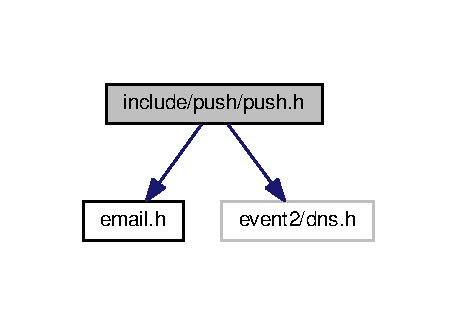
\includegraphics[width=219pt]{push_8h__incl}
\end{center}
\end{figure}
This graph shows which files directly or indirectly include this file\-:
\nopagebreak
\begin{figure}[H]
\begin{center}
\leavevmode
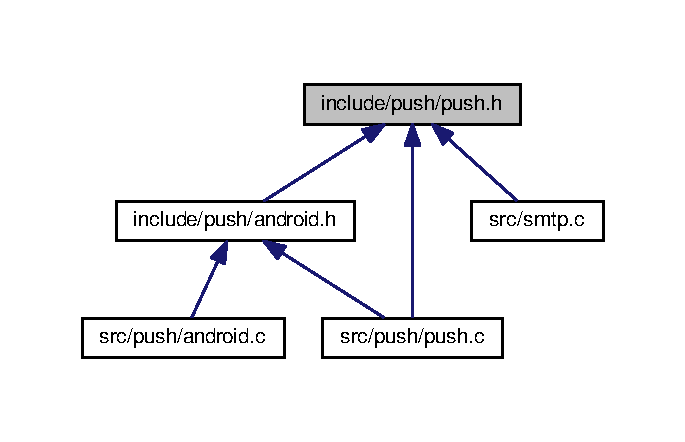
\includegraphics[width=329pt]{push_8h__dep__incl}
\end{center}
\end{figure}
\subsection*{Data Structures}
\begin{DoxyCompactItemize}
\item 
struct \hyperlink{structpush__info}{push\-\_\-info}
\end{DoxyCompactItemize}
\subsection*{Functions}
\begin{DoxyCompactItemize}
\item 
void \hyperlink{push_8h_a69d7cc1b220a09aaeba3079e17822a17}{launch\-\_\-push\-\_\-queries} (char $\ast$address, void $\ast$context, struct \hyperlink{structemail}{email} $\ast$\hyperlink{structemail}{email})
\end{DoxyCompactItemize}
\subsection*{Variables}
\begin{DoxyCompactItemize}
\item 
struct evdns\-\_\-base $\ast$ \hyperlink{push_8h_aa802242597f5727e3390ad90385fd131}{dns}
\end{DoxyCompactItemize}


\subsection{Function Documentation}
\hypertarget{push_8h_a69d7cc1b220a09aaeba3079e17822a17}{\index{push.\-h@{push.\-h}!launch\-\_\-push\-\_\-queries@{launch\-\_\-push\-\_\-queries}}
\index{launch\-\_\-push\-\_\-queries@{launch\-\_\-push\-\_\-queries}!push.h@{push.\-h}}
\subsubsection[{launch\-\_\-push\-\_\-queries}]{\setlength{\rightskip}{0pt plus 5cm}void launch\-\_\-push\-\_\-queries (
\begin{DoxyParamCaption}
\item[{char $\ast$}]{address, }
\item[{void $\ast$}]{context, }
\item[{struct {\bf email} $\ast$}]{email}
\end{DoxyParamCaption}
)}}\label{push_8h_a69d7cc1b220a09aaeba3079e17822a17}


\subsection{Variable Documentation}
\hypertarget{push_8h_aa802242597f5727e3390ad90385fd131}{\index{push.\-h@{push.\-h}!dns@{dns}}
\index{dns@{dns}!push.h@{push.\-h}}
\subsubsection[{dns}]{\setlength{\rightskip}{0pt plus 5cm}struct evdns\-\_\-base$\ast$ dns}}\label{push_8h_aa802242597f5727e3390ad90385fd131}

\hypertarget{safefree_8h}{\section{include/safefree.h File Reference}
\label{safefree_8h}\index{include/safefree.\-h@{include/safefree.\-h}}
}
This graph shows which files directly or indirectly include this file\-:
\nopagebreak
\begin{figure}[H]
\begin{center}
\leavevmode
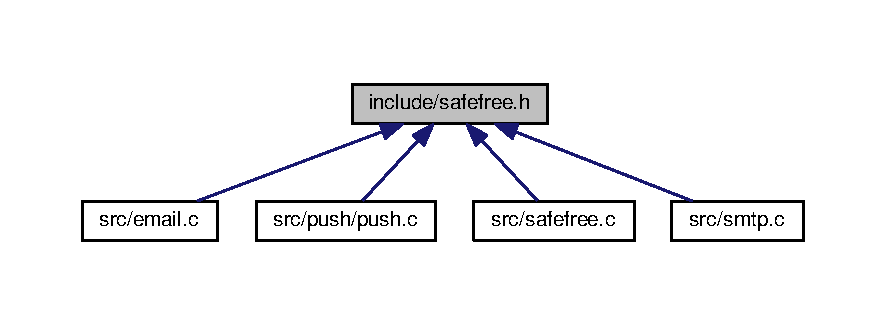
\includegraphics[width=350pt]{safefree_8h__dep__incl}
\end{center}
\end{figure}
\subsection*{Macros}
\begin{DoxyCompactItemize}
\item 
\#define \hyperlink{safefree_8h_a17eef69f501d4a375f9ef6680a2a156e}{S\-A\-F\-E\-F\-R\-E\-E}(p)~\hyperlink{safefree_8c_aa9523f785ef0edb1f61f32f7aa41418c}{safefree}((void$\ast$$\ast$)\&p)
\end{DoxyCompactItemize}
\subsection*{Functions}
\begin{DoxyCompactItemize}
\item 
void \hyperlink{safefree_8h_aa9523f785ef0edb1f61f32f7aa41418c}{safefree} (void $\ast$$\ast$pp)
\end{DoxyCompactItemize}


\subsection{Macro Definition Documentation}
\hypertarget{safefree_8h_a17eef69f501d4a375f9ef6680a2a156e}{\index{safefree.\-h@{safefree.\-h}!S\-A\-F\-E\-F\-R\-E\-E@{S\-A\-F\-E\-F\-R\-E\-E}}
\index{S\-A\-F\-E\-F\-R\-E\-E@{S\-A\-F\-E\-F\-R\-E\-E}!safefree.h@{safefree.\-h}}
\subsubsection[{S\-A\-F\-E\-F\-R\-E\-E}]{\setlength{\rightskip}{0pt plus 5cm}\#define S\-A\-F\-E\-F\-R\-E\-E(
\begin{DoxyParamCaption}
\item[{}]{p}
\end{DoxyParamCaption}
)~{\bf safefree}((void$\ast$$\ast$)\&p)}}\label{safefree_8h_a17eef69f501d4a375f9ef6680a2a156e}


\subsection{Function Documentation}
\hypertarget{safefree_8h_aa9523f785ef0edb1f61f32f7aa41418c}{\index{safefree.\-h@{safefree.\-h}!safefree@{safefree}}
\index{safefree@{safefree}!safefree.h@{safefree.\-h}}
\subsubsection[{safefree}]{\setlength{\rightskip}{0pt plus 5cm}void safefree (
\begin{DoxyParamCaption}
\item[{void $\ast$$\ast$}]{pp}
\end{DoxyParamCaption}
)}}\label{safefree_8h_aa9523f785ef0edb1f61f32f7aa41418c}
A somewhat safe implementation of free, this will set the original passed pointer to N\-U\-L\-L afterwards. Use the macro S\-A\-F\-E\-F\-R\-E\-E so the compiler will shut up about warnings. 
\hypertarget{smtp_8h}{\section{include/smtp.h File Reference}
\label{smtp_8h}\index{include/smtp.\-h@{include/smtp.\-h}}
}
{\ttfamily \#include $<$event.\-h$>$}\\*
Include dependency graph for smtp.\-h\-:
\nopagebreak
\begin{figure}[H]
\begin{center}
\leavevmode
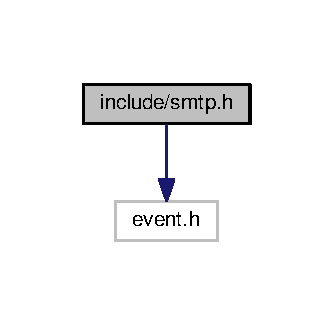
\includegraphics[width=160pt]{smtp_8h__incl}
\end{center}
\end{figure}
This graph shows which files directly or indirectly include this file\-:
\nopagebreak
\begin{figure}[H]
\begin{center}
\leavevmode
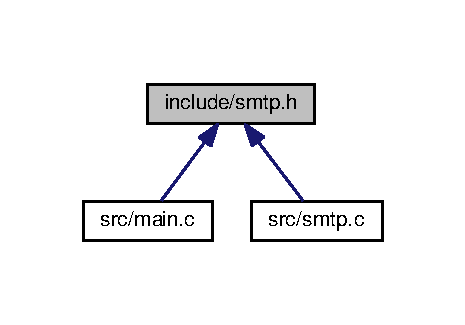
\includegraphics[width=223pt]{smtp_8h__dep__incl}
\end{center}
\end{figure}
\subsection*{Functions}
\begin{DoxyCompactItemize}
\item 
int \hyperlink{smtp_8h_a2cda0186363c8fc3eb7e82796b0159b5}{init\-Mail\-Listener} (struct \hyperlink{main_8c_ac1c1d71aa37cb71608f4f802bb85b200}{event\-\_\-base} $\ast$\hyperlink{main_8c_ac1c1d71aa37cb71608f4f802bb85b200}{event\-\_\-base}, unsigned short listen\-\_\-port)
\item 
void \hyperlink{smtp_8h_a7a834543fbece476c2fed45df76822c0}{close\-Mail\-Listener} ()
\end{DoxyCompactItemize}


\subsection{Function Documentation}
\hypertarget{smtp_8h_a7a834543fbece476c2fed45df76822c0}{\index{smtp.\-h@{smtp.\-h}!close\-Mail\-Listener@{close\-Mail\-Listener}}
\index{close\-Mail\-Listener@{close\-Mail\-Listener}!smtp.h@{smtp.\-h}}
\subsubsection[{close\-Mail\-Listener}]{\setlength{\rightskip}{0pt plus 5cm}void close\-Mail\-Listener (
\begin{DoxyParamCaption}
{}
\end{DoxyParamCaption}
)}}\label{smtp_8h_a7a834543fbece476c2fed45df76822c0}
Close the smtp listener \hypertarget{smtp_8h_a2cda0186363c8fc3eb7e82796b0159b5}{\index{smtp.\-h@{smtp.\-h}!init\-Mail\-Listener@{init\-Mail\-Listener}}
\index{init\-Mail\-Listener@{init\-Mail\-Listener}!smtp.h@{smtp.\-h}}
\subsubsection[{init\-Mail\-Listener}]{\setlength{\rightskip}{0pt plus 5cm}int init\-Mail\-Listener (
\begin{DoxyParamCaption}
\item[{struct {\bf event\-\_\-base} $\ast$}]{event\-\_\-base, }
\item[{unsigned short}]{listen\-\_\-port}
\end{DoxyParamCaption}
)}}\label{smtp_8h_a2cda0186363c8fc3eb7e82796b0159b5}
Init the smtp listener 
\begin{DoxyParams}{Parameters}
{\em event\-\_\-base} & event\-\_\-base to use to listen on \\
\hline
{\em listen\-\_\-port} & port to listen on \\
\hline
\end{DoxyParams}
\begin{DoxyReturn}{Returns}
1 in case we're actually listening 
\end{DoxyReturn}

\hypertarget{string__helpers_8h}{\section{include/string\-\_\-helpers.h File Reference}
\label{string__helpers_8h}\index{include/string\-\_\-helpers.\-h@{include/string\-\_\-helpers.\-h}}
}
This graph shows which files directly or indirectly include this file\-:
\nopagebreak
\begin{figure}[H]
\begin{center}
\leavevmode
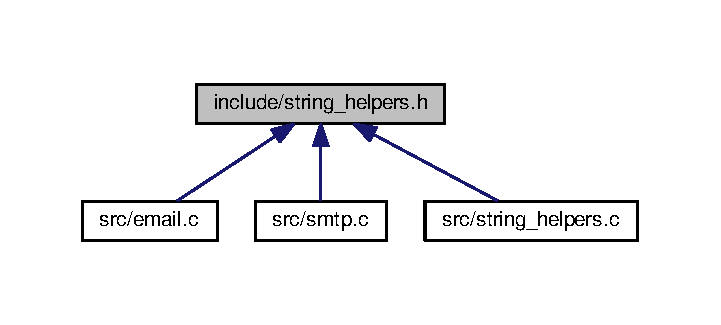
\includegraphics[width=346pt]{string__helpers_8h__dep__incl}
\end{center}
\end{figure}
\subsection*{Functions}
\begin{DoxyCompactItemize}
\item 
int \hyperlink{string__helpers_8h_a8b117c3d470e00b40cc82ec26bc5f3e4}{string\-\_\-starts\-With} (char $\ast$str1, char $\ast$str2)
\item 
int \hyperlink{string__helpers_8h_a6a5539242dc66ee57ed8a30c6bd5979e}{string\-\_\-equals} (char $\ast$str1, char $\ast$str2)
\item 
char $\ast$ \hyperlink{string__helpers_8h_a3ae7aaac50348f5b99fca069b9667bee}{strip\-Out\-Email\-Address} (char $\ast$line)
\item 
int \hyperlink{string__helpers_8h_a20e4e1d1cf8752378fad387f1272fa8d}{string\-\_\-contains} (char $\ast$line, char c)
\item 
int \hyperlink{string__helpers_8h_a358ac995b012642a8d75d63d8f93b122}{valididate\-Email\-Address} (char $\ast$\hyperlink{structemail}{email})
\item 
int \hyperlink{string__helpers_8h_a7b39a32f1f7fdc1f805e61eab1d3f516}{for\-Each\-Character} (char $\ast$input, int($\ast$function)(char input))
\end{DoxyCompactItemize}


\subsection{Function Documentation}
\hypertarget{string__helpers_8h_a7b39a32f1f7fdc1f805e61eab1d3f516}{\index{string\-\_\-helpers.\-h@{string\-\_\-helpers.\-h}!for\-Each\-Character@{for\-Each\-Character}}
\index{for\-Each\-Character@{for\-Each\-Character}!string_helpers.h@{string\-\_\-helpers.\-h}}
\subsubsection[{for\-Each\-Character}]{\setlength{\rightskip}{0pt plus 5cm}int for\-Each\-Character (
\begin{DoxyParamCaption}
\item[{char $\ast$}]{input, }
\item[{int($\ast$)(char input)}]{function}
\end{DoxyParamCaption}
)}}\label{string__helpers_8h_a7b39a32f1f7fdc1f805e61eab1d3f516}
Call a function for each character in a string in case it exits with non-\/zero return that value 
\begin{DoxyParams}{Parameters}
{\em input} & The input string \\
\hline
{\em function} & The function to call for each character \\
\hline
\end{DoxyParams}
\begin{DoxyReturn}{Returns}
Fully depends on function 
\end{DoxyReturn}
\hypertarget{string__helpers_8h_a20e4e1d1cf8752378fad387f1272fa8d}{\index{string\-\_\-helpers.\-h@{string\-\_\-helpers.\-h}!string\-\_\-contains@{string\-\_\-contains}}
\index{string\-\_\-contains@{string\-\_\-contains}!string_helpers.h@{string\-\_\-helpers.\-h}}
\subsubsection[{string\-\_\-contains}]{\setlength{\rightskip}{0pt plus 5cm}int string\-\_\-contains (
\begin{DoxyParamCaption}
\item[{char $\ast$}]{line, }
\item[{char}]{c}
\end{DoxyParamCaption}
)}}\label{string__helpers_8h_a20e4e1d1cf8752378fad387f1272fa8d}
Return if line contains c 
\begin{DoxyParams}{Parameters}
{\em line} & String to check for a certain character \\
\hline
{\em c} & the character to check for \\
\hline
\end{DoxyParams}
\begin{DoxyReturn}{Returns}
1 if line does contain c 
\end{DoxyReturn}
\hypertarget{string__helpers_8h_a6a5539242dc66ee57ed8a30c6bd5979e}{\index{string\-\_\-helpers.\-h@{string\-\_\-helpers.\-h}!string\-\_\-equals@{string\-\_\-equals}}
\index{string\-\_\-equals@{string\-\_\-equals}!string_helpers.h@{string\-\_\-helpers.\-h}}
\subsubsection[{string\-\_\-equals}]{\setlength{\rightskip}{0pt plus 5cm}int string\-\_\-equals (
\begin{DoxyParamCaption}
\item[{char $\ast$}]{str1, }
\item[{char $\ast$}]{str2}
\end{DoxyParamCaption}
)}}\label{string__helpers_8h_a6a5539242dc66ee57ed8a30c6bd5979e}
Simple check if str1 is equal to str2 
\begin{DoxyParams}{Parameters}
{\em str1} & Input string 1 \\
\hline
{\em str2} & Input string 2 \\
\hline
\end{DoxyParams}
\begin{DoxyReturn}{Returns}
It'll return 1 in case they're equal, else it'll return 0 
\end{DoxyReturn}
\hypertarget{string__helpers_8h_a8b117c3d470e00b40cc82ec26bc5f3e4}{\index{string\-\_\-helpers.\-h@{string\-\_\-helpers.\-h}!string\-\_\-starts\-With@{string\-\_\-starts\-With}}
\index{string\-\_\-starts\-With@{string\-\_\-starts\-With}!string_helpers.h@{string\-\_\-helpers.\-h}}
\subsubsection[{string\-\_\-starts\-With}]{\setlength{\rightskip}{0pt plus 5cm}int string\-\_\-starts\-With (
\begin{DoxyParamCaption}
\item[{char $\ast$}]{str1, }
\item[{char $\ast$}]{str2}
\end{DoxyParamCaption}
)}}\label{string__helpers_8h_a8b117c3d470e00b40cc82ec26bc5f3e4}
Simple check if str1 starts with str2 
\begin{DoxyParams}{Parameters}
{\em str1} & Input string \\
\hline
{\em str2} & String line has to start with \\
\hline
\end{DoxyParams}
\begin{DoxyReturn}{Returns}
It'll return 1 in case line does start with start, else it'll return 0 
\end{DoxyReturn}
\hypertarget{string__helpers_8h_a3ae7aaac50348f5b99fca069b9667bee}{\index{string\-\_\-helpers.\-h@{string\-\_\-helpers.\-h}!strip\-Out\-Email\-Address@{strip\-Out\-Email\-Address}}
\index{strip\-Out\-Email\-Address@{strip\-Out\-Email\-Address}!string_helpers.h@{string\-\_\-helpers.\-h}}
\subsubsection[{strip\-Out\-Email\-Address}]{\setlength{\rightskip}{0pt plus 5cm}char$\ast$ strip\-Out\-Email\-Address (
\begin{DoxyParamCaption}
\item[{char $\ast$}]{line}
\end{DoxyParamCaption}
)}}\label{string__helpers_8h_a3ae7aaac50348f5b99fca069b9667bee}
Return just the email address 
\begin{DoxyParams}{Parameters}
{\em line} & Raw line from the S\-M\-T\-P client \\
\hline
\end{DoxyParams}
\begin{DoxyReturn}{Returns}
A new string with just the email address 
\end{DoxyReturn}
\begin{DoxyNote}{Note}
line is not freed. 
\end{DoxyNote}
\hypertarget{string__helpers_8h_a358ac995b012642a8d75d63d8f93b122}{\index{string\-\_\-helpers.\-h@{string\-\_\-helpers.\-h}!valididate\-Email\-Address@{valididate\-Email\-Address}}
\index{valididate\-Email\-Address@{valididate\-Email\-Address}!string_helpers.h@{string\-\_\-helpers.\-h}}
\subsubsection[{valididate\-Email\-Address}]{\setlength{\rightskip}{0pt plus 5cm}int valididate\-Email\-Address (
\begin{DoxyParamCaption}
\item[{char $\ast$}]{email}
\end{DoxyParamCaption}
)}}\label{string__helpers_8h_a358ac995b012642a8d75d63d8f93b122}
Check if this emailaddress contains 1 at sign and is only made up of letters and/or numbers 
\begin{DoxyParams}{Parameters}
{\em email} & The email address to check \\
\hline
\end{DoxyParams}
\begin{DoxyReturn}{Returns}
1 if it's valid 
\end{DoxyReturn}

\hypertarget{email_8c}{\section{src/email.c File Reference}
\label{email_8c}\index{src/email.\-c@{src/email.\-c}}
}
{\ttfamily \#include \char`\"{}email.\-h\char`\"{}}\\*
{\ttfamily \#include \char`\"{}safefree.\-h\char`\"{}}\\*
{\ttfamily \#include \char`\"{}string\-\_\-helpers.\-h\char`\"{}}\\*
{\ttfamily \#include $<$stdlib.\-h$>$}\\*
{\ttfamily \#include $<$string.\-h$>$}\\*
Include dependency graph for email.\-c\-:
\nopagebreak
\begin{figure}[H]
\begin{center}
\leavevmode
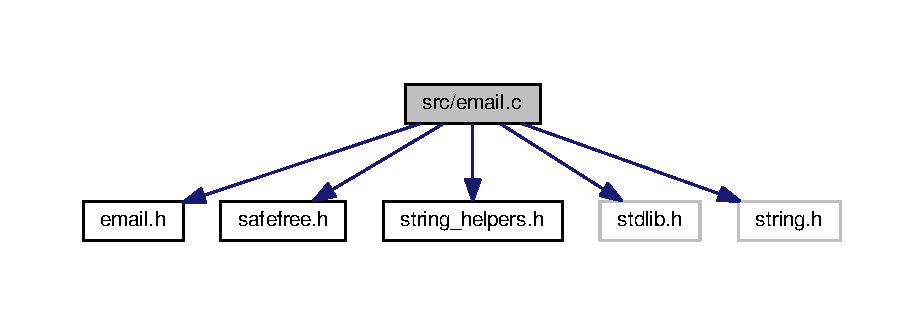
\includegraphics[width=350pt]{email_8c__incl}
\end{center}
\end{figure}
\subsection*{Functions}
\begin{DoxyCompactItemize}
\item 
struct \hyperlink{structemail}{email} $\ast$ \hyperlink{email_8c_a92d36df971c6ea4b807f191461774628}{new\-\_\-email} ()
\item 
void \hyperlink{email_8c_a5227fadfd1014417c4ce6bfc4a925592}{delete\-\_\-email} (struct \hyperlink{structemail}{email} $\ast$\hyperlink{structemail}{email})
\item 
int \hyperlink{email_8c_a21caf89afa30b60df1eec81bfb48e6d0}{email\-\_\-set\-\_\-sender} (struct \hyperlink{structemail}{email} $\ast$\hyperlink{structemail}{email}, char $\ast$from)
\item 
int \hyperlink{email_8c_a634d99bdaba585890305ea9f86312c09}{email\-\_\-add\-\_\-recipient} (struct \hyperlink{structemail}{email} $\ast$\hyperlink{structemail}{email}, char $\ast$to)
\item 
int \hyperlink{email_8c_a46ed54490f60eccc2513cae45ef8adfb}{email\-\_\-has\-\_\-recipients} (struct \hyperlink{structemail}{email} $\ast$\hyperlink{structemail}{email})
\item 
char $\ast$ \hyperlink{email_8c_a8b8b8be04443bcbad35d3100929e2a8f}{email\-\_\-get\-\_\-last\-\_\-recipient} (struct \hyperlink{structemail}{email} $\ast$\hyperlink{structemail}{email})
\item 
int \hyperlink{email_8c_acf2b3d9d17180be215d06b5267bb5042}{email\-\_\-remove\-\_\-email\-\_\-from\-\_\-recipients} (struct \hyperlink{structemail}{email} $\ast$\hyperlink{structemail}{email}, char $\ast$addr)
\item 
int \hyperlink{email_8c_a164bbbf7611e6a4f842a9d9699d756a1}{email\-\_\-set\-\_\-subject} (struct \hyperlink{structemail}{email} $\ast$\hyperlink{structemail}{email}, char $\ast$line)
\item 
void \hyperlink{email_8c_a39795abc038b09b975b2dfaee3067dae}{email\-\_\-for\-\_\-each\-\_\-recipient} (struct \hyperlink{structemail}{email} $\ast$\hyperlink{structemail}{email}, void $\ast$context, void($\ast$execute)(char $\ast$address, void $\ast$context, struct \hyperlink{structemail}{email} $\ast$\hyperlink{structemail}{email}))
\item 
int \hyperlink{email_8c_a179442b2783a7258bfa8e5f69e758a58}{email\-\_\-append\-\_\-data} (struct \hyperlink{structemail}{email} $\ast$\hyperlink{structemail}{email}, char $\ast$data)
\end{DoxyCompactItemize}


\subsection{Function Documentation}
\hypertarget{email_8c_a5227fadfd1014417c4ce6bfc4a925592}{\index{email.\-c@{email.\-c}!delete\-\_\-email@{delete\-\_\-email}}
\index{delete\-\_\-email@{delete\-\_\-email}!email.c@{email.\-c}}
\subsubsection[{delete\-\_\-email}]{\setlength{\rightskip}{0pt plus 5cm}void delete\-\_\-email (
\begin{DoxyParamCaption}
\item[{struct {\bf email} $\ast$}]{email}
\end{DoxyParamCaption}
)}}\label{email_8c_a5227fadfd1014417c4ce6bfc4a925592}
Clean up this email structure 
\begin{DoxyParams}{Parameters}
{\em email} & The email structure we want to clean up \\
\hline
\end{DoxyParams}
\hypertarget{email_8c_a634d99bdaba585890305ea9f86312c09}{\index{email.\-c@{email.\-c}!email\-\_\-add\-\_\-recipient@{email\-\_\-add\-\_\-recipient}}
\index{email\-\_\-add\-\_\-recipient@{email\-\_\-add\-\_\-recipient}!email.c@{email.\-c}}
\subsubsection[{email\-\_\-add\-\_\-recipient}]{\setlength{\rightskip}{0pt plus 5cm}int email\-\_\-add\-\_\-recipient (
\begin{DoxyParamCaption}
\item[{struct {\bf email} $\ast$}]{email, }
\item[{char $\ast$}]{to}
\end{DoxyParamCaption}
)}}\label{email_8c_a634d99bdaba585890305ea9f86312c09}
Add a recipient to our email structure 
\begin{DoxyParams}{Parameters}
{\em email} & The email structure we want to have this recipient \\
\hline
{\em to} & The recipient's email address \\
\hline
\end{DoxyParams}
\begin{DoxyReturn}{Returns}
1 if added correctly, 0 if not added this will only occur when there are more than M\-A\-X\-\_\-\-R\-E\-C\-I\-P\-I\-E\-N\-T\-S recipients or if the email isn't valid 
\end{DoxyReturn}
\hypertarget{email_8c_a179442b2783a7258bfa8e5f69e758a58}{\index{email.\-c@{email.\-c}!email\-\_\-append\-\_\-data@{email\-\_\-append\-\_\-data}}
\index{email\-\_\-append\-\_\-data@{email\-\_\-append\-\_\-data}!email.c@{email.\-c}}
\subsubsection[{email\-\_\-append\-\_\-data}]{\setlength{\rightskip}{0pt plus 5cm}int email\-\_\-append\-\_\-data (
\begin{DoxyParamCaption}
\item[{struct {\bf email} $\ast$}]{email, }
\item[{char $\ast$}]{data}
\end{DoxyParamCaption}
)}}\label{email_8c_a179442b2783a7258bfa8e5f69e758a58}
Parse a raw line to 'append' it to the data field in email 
\begin{DoxyParams}{Parameters}
{\em email} & The email structure we want to have this data \\
\hline
{\em data} & The data we want to append \\
\hline
\end{DoxyParams}
\begin{DoxyReturn}{Returns}
1 in case we're in the right mode, else it'll return 0 
\end{DoxyReturn}
\hypertarget{email_8c_a39795abc038b09b975b2dfaee3067dae}{\index{email.\-c@{email.\-c}!email\-\_\-for\-\_\-each\-\_\-recipient@{email\-\_\-for\-\_\-each\-\_\-recipient}}
\index{email\-\_\-for\-\_\-each\-\_\-recipient@{email\-\_\-for\-\_\-each\-\_\-recipient}!email.c@{email.\-c}}
\subsubsection[{email\-\_\-for\-\_\-each\-\_\-recipient}]{\setlength{\rightskip}{0pt plus 5cm}void email\-\_\-for\-\_\-each\-\_\-recipient (
\begin{DoxyParamCaption}
\item[{struct {\bf email} $\ast$}]{email, }
\item[{void $\ast$}]{context, }
\item[{void($\ast$)(char $\ast$address, void $\ast$context, struct {\bf email} $\ast${\bf email})}]{execute}
\end{DoxyParamCaption}
)}}\label{email_8c_a39795abc038b09b975b2dfaee3067dae}
Execute this function pointer for each recipient 
\begin{DoxyParams}{Parameters}
{\em email} & The email structure to use for the recipients \\
\hline
{\em context} & Void pointer to pass to the function pointer \\
\hline
{\em execute} & The function pointer to execute for each recipient \\
\hline
\end{DoxyParams}
\hypertarget{email_8c_a8b8b8be04443bcbad35d3100929e2a8f}{\index{email.\-c@{email.\-c}!email\-\_\-get\-\_\-last\-\_\-recipient@{email\-\_\-get\-\_\-last\-\_\-recipient}}
\index{email\-\_\-get\-\_\-last\-\_\-recipient@{email\-\_\-get\-\_\-last\-\_\-recipient}!email.c@{email.\-c}}
\subsubsection[{email\-\_\-get\-\_\-last\-\_\-recipient}]{\setlength{\rightskip}{0pt plus 5cm}char$\ast$ email\-\_\-get\-\_\-last\-\_\-recipient (
\begin{DoxyParamCaption}
\item[{struct {\bf email} $\ast$}]{email}
\end{DoxyParamCaption}
)}}\label{email_8c_a8b8b8be04443bcbad35d3100929e2a8f}
Get the last recipient \begin{DoxyReturn}{Returns}
Returns the last recipient in the to array returns N\-U\-L\-L if there are no recipients 
\end{DoxyReturn}
\hypertarget{email_8c_a46ed54490f60eccc2513cae45ef8adfb}{\index{email.\-c@{email.\-c}!email\-\_\-has\-\_\-recipients@{email\-\_\-has\-\_\-recipients}}
\index{email\-\_\-has\-\_\-recipients@{email\-\_\-has\-\_\-recipients}!email.c@{email.\-c}}
\subsubsection[{email\-\_\-has\-\_\-recipients}]{\setlength{\rightskip}{0pt plus 5cm}int email\-\_\-has\-\_\-recipients (
\begin{DoxyParamCaption}
\item[{struct {\bf email} $\ast$}]{email}
\end{DoxyParamCaption}
)}}\label{email_8c_a46ed54490f60eccc2513cae45ef8adfb}
Simple check if the email structure has the from and to field filled in. 
\begin{DoxyParams}{Parameters}
{\em email} & The email structure we want to check for recipients \\
\hline
\end{DoxyParams}
\begin{DoxyReturn}{Returns}
If it has both the from and at least one recipient it'll return 1, else it'll return 0 
\end{DoxyReturn}
\hypertarget{email_8c_acf2b3d9d17180be215d06b5267bb5042}{\index{email.\-c@{email.\-c}!email\-\_\-remove\-\_\-email\-\_\-from\-\_\-recipients@{email\-\_\-remove\-\_\-email\-\_\-from\-\_\-recipients}}
\index{email\-\_\-remove\-\_\-email\-\_\-from\-\_\-recipients@{email\-\_\-remove\-\_\-email\-\_\-from\-\_\-recipients}!email.c@{email.\-c}}
\subsubsection[{email\-\_\-remove\-\_\-email\-\_\-from\-\_\-recipients}]{\setlength{\rightskip}{0pt plus 5cm}int email\-\_\-remove\-\_\-email\-\_\-from\-\_\-recipients (
\begin{DoxyParamCaption}
\item[{struct {\bf email} $\ast$}]{email, }
\item[{char $\ast$}]{addr}
\end{DoxyParamCaption}
)}}\label{email_8c_acf2b3d9d17180be215d06b5267bb5042}
Remove an email address from the mail structure 
\begin{DoxyParams}{Parameters}
{\em email} & The structure to remove an address from \\
\hline
{\em addr} & T\-He address to remove \\
\hline
\end{DoxyParams}
\begin{DoxyReturn}{Returns}
1 in case there was something deleted, else it'll return 0 
\end{DoxyReturn}
\hypertarget{email_8c_a21caf89afa30b60df1eec81bfb48e6d0}{\index{email.\-c@{email.\-c}!email\-\_\-set\-\_\-sender@{email\-\_\-set\-\_\-sender}}
\index{email\-\_\-set\-\_\-sender@{email\-\_\-set\-\_\-sender}!email.c@{email.\-c}}
\subsubsection[{email\-\_\-set\-\_\-sender}]{\setlength{\rightskip}{0pt plus 5cm}int email\-\_\-set\-\_\-sender (
\begin{DoxyParamCaption}
\item[{struct {\bf email} $\ast$}]{email, }
\item[{char $\ast$}]{from}
\end{DoxyParamCaption}
)}}\label{email_8c_a21caf89afa30b60df1eec81bfb48e6d0}
Set our sender 
\begin{DoxyParams}{Parameters}
{\em email} & The email structure we want to have this sender \\
\hline
{\em from} & The sender's email address \\
\hline
\end{DoxyParams}
\begin{DoxyReturn}{Returns}
1 in case we set it correctly, else we'll return 0 
\end{DoxyReturn}
\hypertarget{email_8c_a164bbbf7611e6a4f842a9d9699d756a1}{\index{email.\-c@{email.\-c}!email\-\_\-set\-\_\-subject@{email\-\_\-set\-\_\-subject}}
\index{email\-\_\-set\-\_\-subject@{email\-\_\-set\-\_\-subject}!email.c@{email.\-c}}
\subsubsection[{email\-\_\-set\-\_\-subject}]{\setlength{\rightskip}{0pt plus 5cm}int email\-\_\-set\-\_\-subject (
\begin{DoxyParamCaption}
\item[{struct {\bf email} $\ast$}]{email, }
\item[{char $\ast$}]{line}
\end{DoxyParamCaption}
)}}\label{email_8c_a164bbbf7611e6a4f842a9d9699d756a1}
Parse the subject and set it to the email structure 
\begin{DoxyParams}{Parameters}
{\em email} & The email structure we want to have the subject \\
\hline
{\em line} & The raw smtp line to parse for the subject \\
\hline
\end{DoxyParams}
\begin{DoxyReturn}{Returns}
1 in case there is a subject set, else it'll return 0 
\end{DoxyReturn}
\hypertarget{email_8c_a92d36df971c6ea4b807f191461774628}{\index{email.\-c@{email.\-c}!new\-\_\-email@{new\-\_\-email}}
\index{new\-\_\-email@{new\-\_\-email}!email.c@{email.\-c}}
\subsubsection[{new\-\_\-email}]{\setlength{\rightskip}{0pt plus 5cm}struct {\bf email}$\ast$ new\-\_\-email (
\begin{DoxyParamCaption}
{}
\end{DoxyParamCaption}
)\hspace{0.3cm}{\ttfamily [read]}}}\label{email_8c_a92d36df971c6ea4b807f191461774628}
Create a new email structure and return this \begin{DoxyReturn}{Returns}
a new email structure 
\end{DoxyReturn}

\hypertarget{main_8c}{\section{src/main.c File Reference}
\label{main_8c}\index{src/main.\-c@{src/main.\-c}}
}
{\ttfamily \#include \char`\"{}log.\-h\char`\"{}}\\*
{\ttfamily \#include \char`\"{}smtp.\-h\char`\"{}}\\*
{\ttfamily \#include \char`\"{}postgres.\-h\char`\"{}}\\*
{\ttfamily \#include $<$event.\-h$>$}\\*
{\ttfamily \#include $<$signal.\-h$>$}\\*
{\ttfamily \#include $<$getopt.\-h$>$}\\*
{\ttfamily \#include $<$limits.\-h$>$}\\*
{\ttfamily \#include $<$unistd.\-h$>$}\\*
{\ttfamily \#include $<$openssl/ssl.\-h$>$}\\*
{\ttfamily \#include $<$openssl/err.\-h$>$}\\*
Include dependency graph for main.\-c\-:
\nopagebreak
\begin{figure}[H]
\begin{center}
\leavevmode
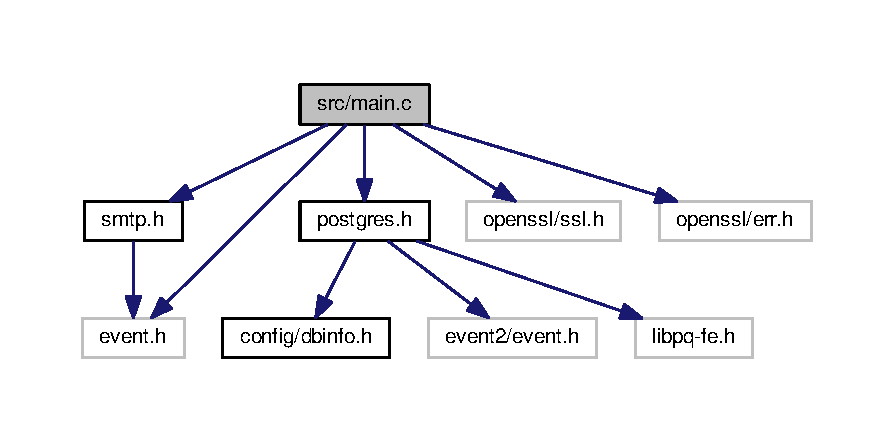
\includegraphics[width=350pt]{main_8c__incl}
\end{center}
\end{figure}
\subsection*{Functions}
\begin{DoxyCompactItemize}
\item 
void \hyperlink{main_8c_aeec856fa74dd34d7ca6374d638c27b20}{on\-Signal} (int signal)
\item 
void \hyperlink{main_8c_a2ef30c42cbc289d899a8be5d2d8f77d0}{usage} ()
\item 
int \hyperlink{main_8c_a3c04138a5bfe5d72780bb7e82a18e627}{main} (int argc, char $\ast$$\ast$argv)
\end{DoxyCompactItemize}
\subsection*{Variables}
\begin{DoxyCompactItemize}
\item 
struct event\-\_\-base $\ast$ \hyperlink{main_8c_ac1c1d71aa37cb71608f4f802bb85b200}{event\-\_\-base} = N\-U\-L\-L
\end{DoxyCompactItemize}


\subsection{Function Documentation}
\hypertarget{main_8c_a3c04138a5bfe5d72780bb7e82a18e627}{\index{main.\-c@{main.\-c}!main@{main}}
\index{main@{main}!main.c@{main.\-c}}
\subsubsection[{main}]{\setlength{\rightskip}{0pt plus 5cm}int main (
\begin{DoxyParamCaption}
\item[{int}]{argc, }
\item[{char $\ast$$\ast$}]{argv}
\end{DoxyParamCaption}
)}}\label{main_8c_a3c04138a5bfe5d72780bb7e82a18e627}
\hypertarget{main_8c_aeec856fa74dd34d7ca6374d638c27b20}{\index{main.\-c@{main.\-c}!on\-Signal@{on\-Signal}}
\index{on\-Signal@{on\-Signal}!main.c@{main.\-c}}
\subsubsection[{on\-Signal}]{\setlength{\rightskip}{0pt plus 5cm}void on\-Signal (
\begin{DoxyParamCaption}
\item[{int}]{signal}
\end{DoxyParamCaption}
)}}\label{main_8c_aeec856fa74dd34d7ca6374d638c27b20}
\hypertarget{main_8c_a2ef30c42cbc289d899a8be5d2d8f77d0}{\index{main.\-c@{main.\-c}!usage@{usage}}
\index{usage@{usage}!main.c@{main.\-c}}
\subsubsection[{usage}]{\setlength{\rightskip}{0pt plus 5cm}void usage (
\begin{DoxyParamCaption}
{}
\end{DoxyParamCaption}
)}}\label{main_8c_a2ef30c42cbc289d899a8be5d2d8f77d0}


\subsection{Variable Documentation}
\hypertarget{main_8c_ac1c1d71aa37cb71608f4f802bb85b200}{\index{main.\-c@{main.\-c}!event\-\_\-base@{event\-\_\-base}}
\index{event\-\_\-base@{event\-\_\-base}!main.c@{main.\-c}}
\subsubsection[{event\-\_\-base}]{\setlength{\rightskip}{0pt plus 5cm}struct event\-\_\-base$\ast$ event\-\_\-base = N\-U\-L\-L}}\label{main_8c_ac1c1d71aa37cb71608f4f802bb85b200}

\hypertarget{postgres_8c}{\section{src/postgres.c File Reference}
\label{postgres_8c}\index{src/postgres.\-c@{src/postgres.\-c}}
}
{\ttfamily \#include \char`\"{}postgres.\-h\char`\"{}}\\*
{\ttfamily \#include $<$event2/bufferevent.\-h$>$}\\*
{\ttfamily \#include $<$event2/event\-\_\-struct.\-h$>$}\\*
{\ttfamily \#include $<$limits.\-h$>$}\\*
{\ttfamily \#include $<$stdlib.\-h$>$}\\*
Include dependency graph for postgres.\-c\-:
\nopagebreak
\begin{figure}[H]
\begin{center}
\leavevmode
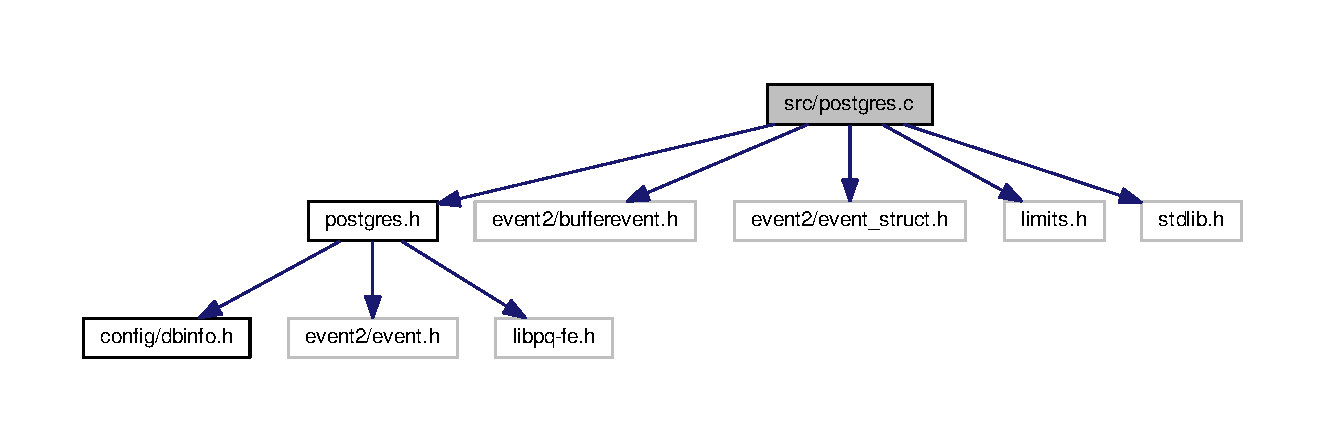
\includegraphics[width=350pt]{postgres_8c__incl}
\end{center}
\end{figure}
\subsection*{Data Structures}
\begin{DoxyCompactItemize}
\item 
struct \hyperlink{structquery__struct}{query\-\_\-struct}
\item 
struct \hyperlink{structconnection__struct}{connection\-\_\-struct}
\end{DoxyCompactItemize}
\subsection*{Functions}
\begin{DoxyCompactItemize}
\item 
void \hyperlink{postgres_8c_ad2d8d5718324b20d939a4b04cd3131ff}{init\-Database\-Pool} (struct event\-\_\-base $\ast$base)
\item 
void \hyperlink{postgres_8c_a7ffcffb58bb853dde98160e1e4546f2c}{append\-Query\-Pool} (struct \hyperlink{structconnection__struct}{connection\-\_\-struct} $\ast$conn, struct \hyperlink{structquery__struct}{query\-\_\-struct} $\ast$query)
\item 
int \hyperlink{postgres_8c_a953a5303803fe3ab05decb3c4c7db8a8}{database\-Query} (char $\ast$query, void($\ast$callback)(P\-Gresult $\ast$, void $\ast$, char $\ast$), void $\ast$context)
\end{DoxyCompactItemize}
\subsection*{Variables}
\begin{DoxyCompactItemize}
\item 
struct \hyperlink{structconnection__struct}{connection\-\_\-struct} $\ast$ \hyperlink{postgres_8c_a411f331390d3a9823bad89d2521a48e2}{database\-Pool} \mbox{[}\hyperlink{postgres_8h_a053b7859476cc9867ec62c49e68d3fa1}{M\-A\-X\-\_\-\-C\-O\-N\-N\-E\-C\-T\-I\-O\-N\-S}\mbox{]}
\end{DoxyCompactItemize}


\subsection{Function Documentation}
\hypertarget{postgres_8c_a7ffcffb58bb853dde98160e1e4546f2c}{\index{postgres.\-c@{postgres.\-c}!append\-Query\-Pool@{append\-Query\-Pool}}
\index{append\-Query\-Pool@{append\-Query\-Pool}!postgres.c@{postgres.\-c}}
\subsubsection[{append\-Query\-Pool}]{\setlength{\rightskip}{0pt plus 5cm}void append\-Query\-Pool (
\begin{DoxyParamCaption}
\item[{struct {\bf connection\-\_\-struct} $\ast$}]{conn, }
\item[{struct {\bf query\-\_\-struct} $\ast$}]{query}
\end{DoxyParamCaption}
)}}\label{postgres_8c_a7ffcffb58bb853dde98160e1e4546f2c}
\hypertarget{postgres_8c_a953a5303803fe3ab05decb3c4c7db8a8}{\index{postgres.\-c@{postgres.\-c}!database\-Query@{database\-Query}}
\index{database\-Query@{database\-Query}!postgres.c@{postgres.\-c}}
\subsubsection[{database\-Query}]{\setlength{\rightskip}{0pt plus 5cm}int database\-Query (
\begin{DoxyParamCaption}
\item[{char $\ast$}]{query, }
\item[{void($\ast$)(P\-Gresult $\ast$, void $\ast$, char $\ast$)}]{callback, }
\item[{void $\ast$}]{context}
\end{DoxyParamCaption}
)}}\label{postgres_8c_a953a5303803fe3ab05decb3c4c7db8a8}
\hypertarget{postgres_8c_ad2d8d5718324b20d939a4b04cd3131ff}{\index{postgres.\-c@{postgres.\-c}!init\-Database\-Pool@{init\-Database\-Pool}}
\index{init\-Database\-Pool@{init\-Database\-Pool}!postgres.c@{postgres.\-c}}
\subsubsection[{init\-Database\-Pool}]{\setlength{\rightskip}{0pt plus 5cm}void init\-Database\-Pool (
\begin{DoxyParamCaption}
\item[{struct event\-\_\-base $\ast$}]{base}
\end{DoxyParamCaption}
)}}\label{postgres_8c_ad2d8d5718324b20d939a4b04cd3131ff}


\subsection{Variable Documentation}
\hypertarget{postgres_8c_a411f331390d3a9823bad89d2521a48e2}{\index{postgres.\-c@{postgres.\-c}!database\-Pool@{database\-Pool}}
\index{database\-Pool@{database\-Pool}!postgres.c@{postgres.\-c}}
\subsubsection[{database\-Pool}]{\setlength{\rightskip}{0pt plus 5cm}struct {\bf connection\-\_\-struct}$\ast$ database\-Pool\mbox{[}{\bf M\-A\-X\-\_\-\-C\-O\-N\-N\-E\-C\-T\-I\-O\-N\-S}\mbox{]}}}\label{postgres_8c_a411f331390d3a9823bad89d2521a48e2}

\hypertarget{android_8c}{\section{src/push/android.c File Reference}
\label{android_8c}\index{src/push/android.\-c@{src/push/android.\-c}}
}
{\ttfamily \#include \char`\"{}push/android.\-h\char`\"{}}\\*
{\ttfamily \#include \char`\"{}config/gcm\-\_\-key.\-h\char`\"{}}\\*
{\ttfamily \#include $<$openssl/ssl.\-h$>$}\\*
{\ttfamily \#include $<$event2/dns.\-h$>$}\\*
{\ttfamily \#include $<$event2/buffer.\-h$>$}\\*
{\ttfamily \#include $<$event2/bufferevent.\-h$>$}\\*
{\ttfamily \#include $<$event2/bufferevent\-\_\-ssl.\-h$>$}\\*
Include dependency graph for android.\-c\-:
\nopagebreak
\begin{figure}[H]
\begin{center}
\leavevmode
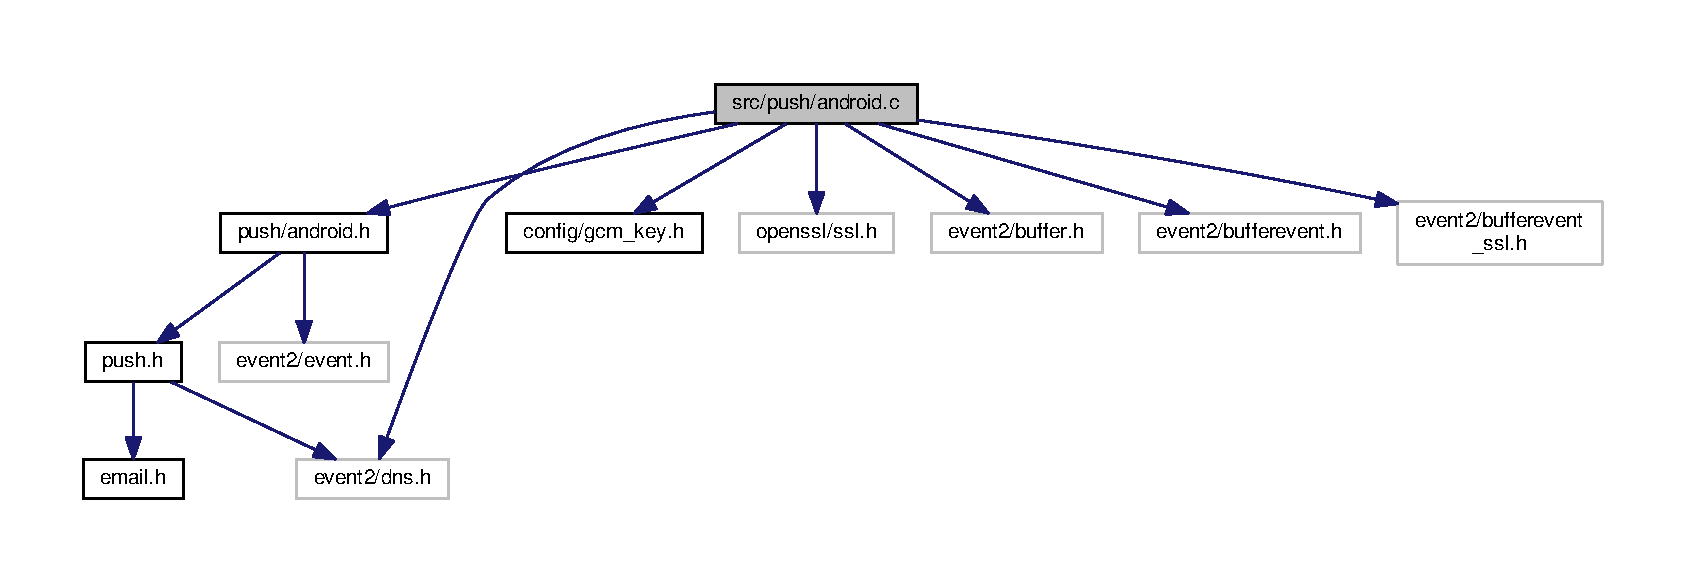
\includegraphics[width=350pt]{android_8c__incl}
\end{center}
\end{figure}
\subsection*{Functions}
\begin{DoxyCompactItemize}
\item 
void \hyperlink{android_8c_a9057dbf56736a0461560bdca4d0eba4c}{android\-\_\-push} (struct \hyperlink{structpush__info}{push\-\_\-info} $\ast$\hyperlink{structpush__info}{push\-\_\-info}, char $\ast$push\-\_\-id, struct \hyperlink{main_8c_ac1c1d71aa37cb71608f4f802bb85b200}{event\-\_\-base} $\ast$\hyperlink{main_8c_ac1c1d71aa37cb71608f4f802bb85b200}{event\-\_\-base})
\end{DoxyCompactItemize}


\subsection{Function Documentation}
\hypertarget{android_8c_a9057dbf56736a0461560bdca4d0eba4c}{\index{android.\-c@{android.\-c}!android\-\_\-push@{android\-\_\-push}}
\index{android\-\_\-push@{android\-\_\-push}!android.c@{android.\-c}}
\subsubsection[{android\-\_\-push}]{\setlength{\rightskip}{0pt plus 5cm}void android\-\_\-push (
\begin{DoxyParamCaption}
\item[{struct {\bf push\-\_\-info} $\ast$}]{push\-\_\-info, }
\item[{char $\ast$}]{push\-\_\-id, }
\item[{struct {\bf event\-\_\-base} $\ast$}]{event\-\_\-base}
\end{DoxyParamCaption}
)}}\label{android_8c_a9057dbf56736a0461560bdca4d0eba4c}

\hypertarget{push_8c}{\section{src/push/push.c File Reference}
\label{push_8c}\index{src/push/push.\-c@{src/push/push.\-c}}
}
{\ttfamily \#include \char`\"{}push/push.\-h\char`\"{}}\\*
{\ttfamily \#include \char`\"{}postgres.\-h\char`\"{}}\\*
{\ttfamily \#include \char`\"{}safefree.\-h\char`\"{}}\\*
{\ttfamily \#include $<$stdlib.\-h$>$}\\*
{\ttfamily \#include $<$string.\-h$>$}\\*
{\ttfamily \#include \char`\"{}push/android.\-h\char`\"{}}\\*
Include dependency graph for push.\-c\-:
\nopagebreak
\begin{figure}[H]
\begin{center}
\leavevmode
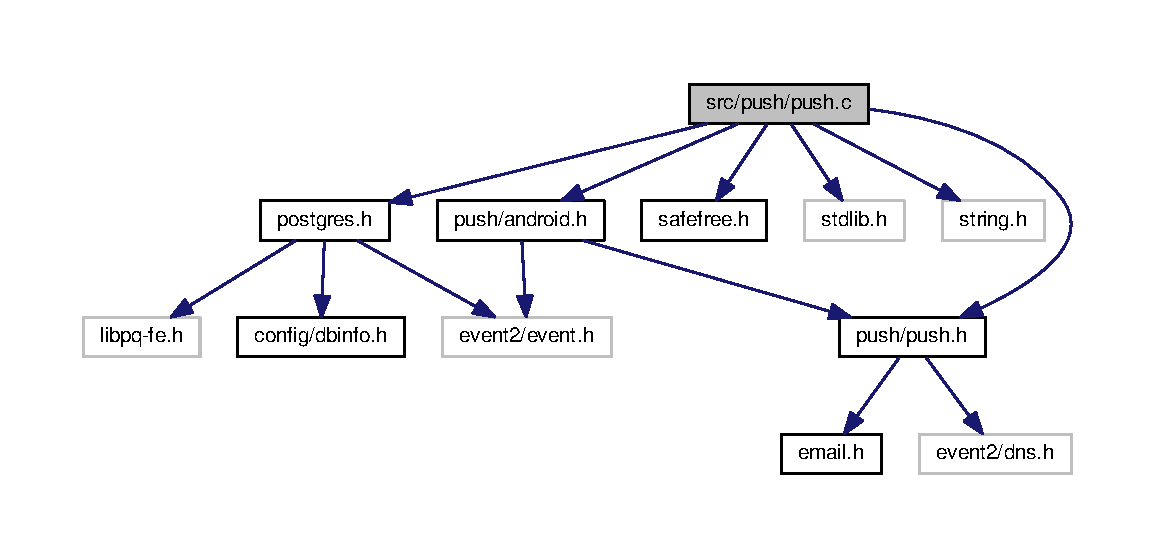
\includegraphics[width=350pt]{push_8c__incl}
\end{center}
\end{figure}
\subsection*{Functions}
\begin{DoxyCompactItemize}
\item 
void \hyperlink{push_8c_a69d7cc1b220a09aaeba3079e17822a17}{launch\-\_\-push\-\_\-queries} (char $\ast$address, void $\ast$context, struct \hyperlink{structemail}{email} $\ast$\hyperlink{structemail}{email})
\item 
int \hyperlink{push_8c_aba2da5d318bc3231b4e607788ab7b400}{amount\-\_\-of\-\_\-push\-\_\-functions} ()
\end{DoxyCompactItemize}
\subsection*{Variables}
\begin{DoxyCompactItemize}
\item 
struct evdns\-\_\-base $\ast$ \hyperlink{push_8c_aa802242597f5727e3390ad90385fd131}{dns} = N\-U\-L\-L
\item 
void($\ast$ \hyperlink{push_8c_ad0d68c8313631ea37c9cd78ec8659e40}{push\-\_\-functions} \mbox{[}$\,$\mbox{]})(struct \hyperlink{structpush__info}{push\-\_\-info} $\ast$, char $\ast$, struct \hyperlink{main_8c_ac1c1d71aa37cb71608f4f802bb85b200}{event\-\_\-base} $\ast$)
\end{DoxyCompactItemize}


\subsection{Function Documentation}
\hypertarget{push_8c_aba2da5d318bc3231b4e607788ab7b400}{\index{push.\-c@{push.\-c}!amount\-\_\-of\-\_\-push\-\_\-functions@{amount\-\_\-of\-\_\-push\-\_\-functions}}
\index{amount\-\_\-of\-\_\-push\-\_\-functions@{amount\-\_\-of\-\_\-push\-\_\-functions}!push.c@{push.\-c}}
\subsubsection[{amount\-\_\-of\-\_\-push\-\_\-functions}]{\setlength{\rightskip}{0pt plus 5cm}int amount\-\_\-of\-\_\-push\-\_\-functions (
\begin{DoxyParamCaption}
{}
\end{DoxyParamCaption}
)}}\label{push_8c_aba2da5d318bc3231b4e607788ab7b400}
\hypertarget{push_8c_a69d7cc1b220a09aaeba3079e17822a17}{\index{push.\-c@{push.\-c}!launch\-\_\-push\-\_\-queries@{launch\-\_\-push\-\_\-queries}}
\index{launch\-\_\-push\-\_\-queries@{launch\-\_\-push\-\_\-queries}!push.c@{push.\-c}}
\subsubsection[{launch\-\_\-push\-\_\-queries}]{\setlength{\rightskip}{0pt plus 5cm}void launch\-\_\-push\-\_\-queries (
\begin{DoxyParamCaption}
\item[{char $\ast$}]{address, }
\item[{void $\ast$}]{context, }
\item[{struct {\bf email} $\ast$}]{email}
\end{DoxyParamCaption}
)}}\label{push_8c_a69d7cc1b220a09aaeba3079e17822a17}


\subsection{Variable Documentation}
\hypertarget{push_8c_aa802242597f5727e3390ad90385fd131}{\index{push.\-c@{push.\-c}!dns@{dns}}
\index{dns@{dns}!push.c@{push.\-c}}
\subsubsection[{dns}]{\setlength{\rightskip}{0pt plus 5cm}struct evdns\-\_\-base$\ast$ dns = N\-U\-L\-L}}\label{push_8c_aa802242597f5727e3390ad90385fd131}
\hypertarget{push_8c_ad0d68c8313631ea37c9cd78ec8659e40}{\index{push.\-c@{push.\-c}!push\-\_\-functions@{push\-\_\-functions}}
\index{push\-\_\-functions@{push\-\_\-functions}!push.c@{push.\-c}}
\subsubsection[{push\-\_\-functions}]{\setlength{\rightskip}{0pt plus 5cm}void($\ast$ push\-\_\-functions\mbox{[}$\,$\mbox{]})(struct {\bf push\-\_\-info} $\ast$, char $\ast$, struct {\bf event\-\_\-base} $\ast$)}}\label{push_8c_ad0d68c8313631ea37c9cd78ec8659e40}
{\bfseries Initial value\-:}
\begin{DoxyCode}
= \{
  \hyperlink{android_8h_a9057dbf56736a0461560bdca4d0eba4c}{android\_push},
  NULL
\}
\end{DoxyCode}

\hypertarget{safefree_8c}{\section{src/safefree.c File Reference}
\label{safefree_8c}\index{src/safefree.\-c@{src/safefree.\-c}}
}
{\ttfamily \#include \char`\"{}safefree.\-h\char`\"{}}\\*
{\ttfamily \#include $<$stdlib.\-h$>$}\\*
Include dependency graph for safefree.\-c\-:
\nopagebreak
\begin{figure}[H]
\begin{center}
\leavevmode
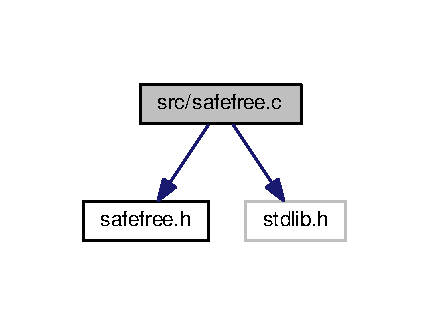
\includegraphics[width=206pt]{safefree_8c__incl}
\end{center}
\end{figure}
\subsection*{Functions}
\begin{DoxyCompactItemize}
\item 
void \hyperlink{safefree_8c_aa9523f785ef0edb1f61f32f7aa41418c}{safefree} (void $\ast$$\ast$pp)
\end{DoxyCompactItemize}


\subsection{Function Documentation}
\hypertarget{safefree_8c_aa9523f785ef0edb1f61f32f7aa41418c}{\index{safefree.\-c@{safefree.\-c}!safefree@{safefree}}
\index{safefree@{safefree}!safefree.c@{safefree.\-c}}
\subsubsection[{safefree}]{\setlength{\rightskip}{0pt plus 5cm}void safefree (
\begin{DoxyParamCaption}
\item[{void $\ast$$\ast$}]{pp}
\end{DoxyParamCaption}
)}}\label{safefree_8c_aa9523f785ef0edb1f61f32f7aa41418c}

\hypertarget{smtp_8c}{\section{src/smtp.c File Reference}
\label{smtp_8c}\index{src/smtp.\-c@{src/smtp.\-c}}
}
{\ttfamily \#include \char`\"{}smtp.\-h\char`\"{}}\\*
{\ttfamily \#include \char`\"{}log.\-h\char`\"{}}\\*
{\ttfamily \#include \char`\"{}email.\-h\char`\"{}}\\*
{\ttfamily \#include \char`\"{}safefree.\-h\char`\"{}}\\*
{\ttfamily \#include \char`\"{}push/push.\-h\char`\"{}}\\*
{\ttfamily \#include \char`\"{}string\-\_\-helpers.\-h\char`\"{}}\\*
{\ttfamily \#include $<$event2/listener.\-h$>$}\\*
{\ttfamily \#include $<$ctype.\-h$>$}\\*
{\ttfamily \#include $<$stdio.\-h$>$}\\*
{\ttfamily \#include $<$fcntl.\-h$>$}\\*
{\ttfamily \#include $<$stdlib.\-h$>$}\\*
{\ttfamily \#include $<$string.\-h$>$}\\*
{\ttfamily \#include $<$unistd.\-h$>$}\\*
{\ttfamily \#include \char`\"{}postgres.\-h\char`\"{}}\\*
Include dependency graph for smtp.\-c\-:
\nopagebreak
\begin{figure}[H]
\begin{center}
\leavevmode
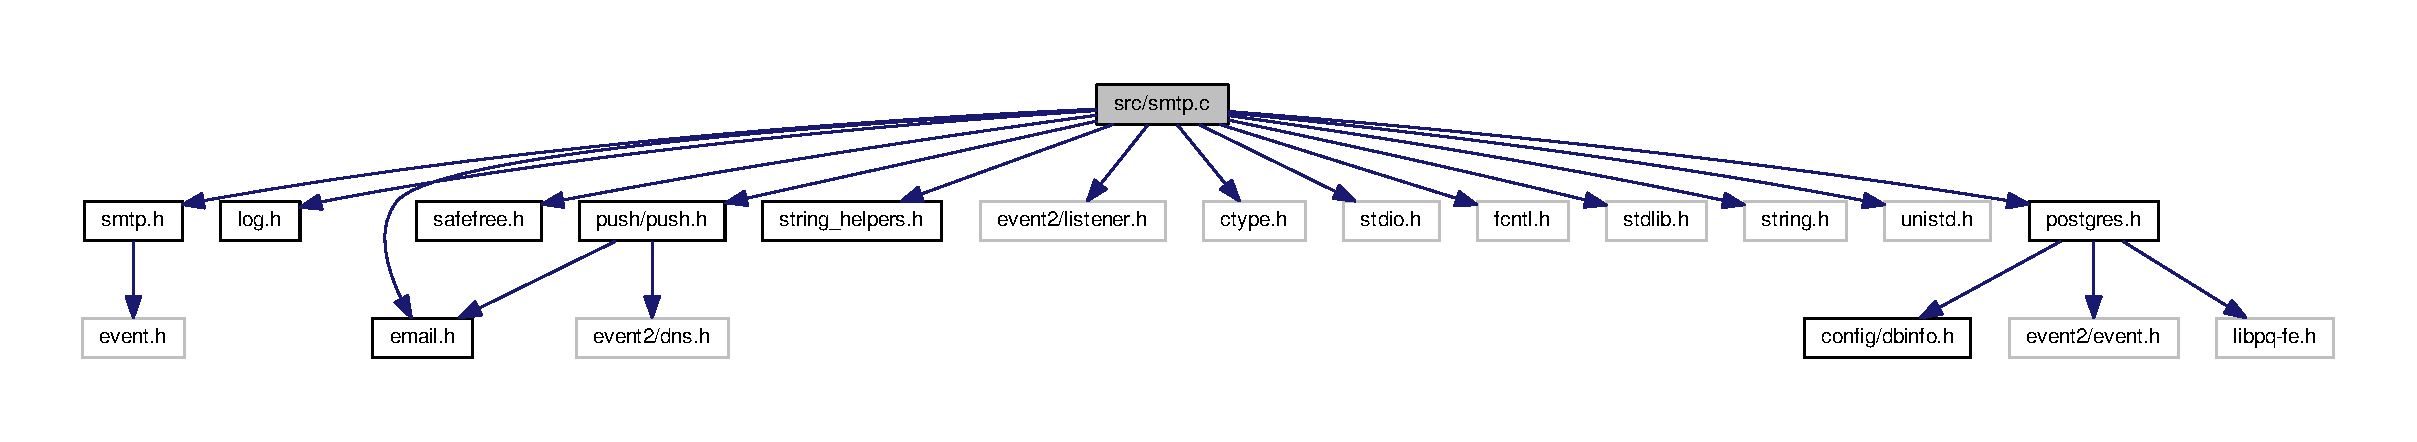
\includegraphics[width=350pt]{smtp_8c__incl}
\end{center}
\end{figure}
\subsection*{Macros}
\begin{DoxyCompactItemize}
\item 
\#define \hyperlink{smtp_8c_a36a3eeada74bd9dc4bf4e95ff8d2c8e8}{F\-R\-O\-M\-\_\-\-Q\-U\-E\-R\-Y\-\_\-\-S\-T\-A\-R\-T}~45
\item 
\#define \hyperlink{smtp_8c_abb57f9d72e6456d89e85581dba4ef84a}{F\-R\-O\-M\-\_\-\-Q\-U\-E\-R\-Y\-\_\-\-E\-N\-D}~10
\item 
\#define \hyperlink{smtp_8c_a747c9399c82c88a86663d09ebce6f5a3}{T\-O\-\_\-\-Q\-U\-E\-R\-Y\-\_\-\-S\-T\-A\-R\-T}~38
\item 
\#define \hyperlink{smtp_8c_a1f8c2f1b27052fa6e8adf07b7375801d}{T\-O\-\_\-\-Q\-U\-E\-R\-Y\-\_\-\-E\-N\-D}~10
\end{DoxyCompactItemize}
\subsection*{Functions}
\begin{DoxyCompactItemize}
\item 
int \hyperlink{smtp_8c_a2cda0186363c8fc3eb7e82796b0159b5}{init\-Mail\-Listener} (struct \hyperlink{main_8c_ac1c1d71aa37cb71608f4f802bb85b200}{event\-\_\-base} $\ast$\hyperlink{main_8c_ac1c1d71aa37cb71608f4f802bb85b200}{event\-\_\-base}, unsigned short listen\-\_\-port)
\item 
void \hyperlink{smtp_8c_a7a834543fbece476c2fed45df76822c0}{close\-Mail\-Listener} ()
\item 
char $\ast$ \hyperlink{smtp_8c_ab63f83e9df29bdad3881cb2c3aa03724}{create\-\_\-check\-\_\-email\-\_\-from\-\_\-query} (char $\ast$\hyperlink{structemail}{email})
\item 
char $\ast$ \hyperlink{smtp_8c_ab1566ddf190846a916c1295fe5ee8f14}{create\-\_\-check\-\_\-email\-\_\-to\-\_\-query} (char $\ast$\hyperlink{structemail}{email})
\item 
int \hyperlink{smtp_8c_a91ed65212973d3dc30e865bd324c50f5}{is\-Email\-Characters} (char c)
\end{DoxyCompactItemize}
\subsection*{Variables}
\begin{DoxyCompactItemize}
\item 
struct evconnlistener $\ast$ \hyperlink{smtp_8c_a0fb084a5ef4d5874db805c2df1375d7b}{listener}
\end{DoxyCompactItemize}


\subsection{Macro Definition Documentation}
\hypertarget{smtp_8c_abb57f9d72e6456d89e85581dba4ef84a}{\index{smtp.\-c@{smtp.\-c}!F\-R\-O\-M\-\_\-\-Q\-U\-E\-R\-Y\-\_\-\-E\-N\-D@{F\-R\-O\-M\-\_\-\-Q\-U\-E\-R\-Y\-\_\-\-E\-N\-D}}
\index{F\-R\-O\-M\-\_\-\-Q\-U\-E\-R\-Y\-\_\-\-E\-N\-D@{F\-R\-O\-M\-\_\-\-Q\-U\-E\-R\-Y\-\_\-\-E\-N\-D}!smtp.c@{smtp.\-c}}
\subsubsection[{F\-R\-O\-M\-\_\-\-Q\-U\-E\-R\-Y\-\_\-\-E\-N\-D}]{\setlength{\rightskip}{0pt plus 5cm}\#define F\-R\-O\-M\-\_\-\-Q\-U\-E\-R\-Y\-\_\-\-E\-N\-D~10}}\label{smtp_8c_abb57f9d72e6456d89e85581dba4ef84a}
\hypertarget{smtp_8c_a36a3eeada74bd9dc4bf4e95ff8d2c8e8}{\index{smtp.\-c@{smtp.\-c}!F\-R\-O\-M\-\_\-\-Q\-U\-E\-R\-Y\-\_\-\-S\-T\-A\-R\-T@{F\-R\-O\-M\-\_\-\-Q\-U\-E\-R\-Y\-\_\-\-S\-T\-A\-R\-T}}
\index{F\-R\-O\-M\-\_\-\-Q\-U\-E\-R\-Y\-\_\-\-S\-T\-A\-R\-T@{F\-R\-O\-M\-\_\-\-Q\-U\-E\-R\-Y\-\_\-\-S\-T\-A\-R\-T}!smtp.c@{smtp.\-c}}
\subsubsection[{F\-R\-O\-M\-\_\-\-Q\-U\-E\-R\-Y\-\_\-\-S\-T\-A\-R\-T}]{\setlength{\rightskip}{0pt plus 5cm}\#define F\-R\-O\-M\-\_\-\-Q\-U\-E\-R\-Y\-\_\-\-S\-T\-A\-R\-T~45}}\label{smtp_8c_a36a3eeada74bd9dc4bf4e95ff8d2c8e8}
\hypertarget{smtp_8c_a1f8c2f1b27052fa6e8adf07b7375801d}{\index{smtp.\-c@{smtp.\-c}!T\-O\-\_\-\-Q\-U\-E\-R\-Y\-\_\-\-E\-N\-D@{T\-O\-\_\-\-Q\-U\-E\-R\-Y\-\_\-\-E\-N\-D}}
\index{T\-O\-\_\-\-Q\-U\-E\-R\-Y\-\_\-\-E\-N\-D@{T\-O\-\_\-\-Q\-U\-E\-R\-Y\-\_\-\-E\-N\-D}!smtp.c@{smtp.\-c}}
\subsubsection[{T\-O\-\_\-\-Q\-U\-E\-R\-Y\-\_\-\-E\-N\-D}]{\setlength{\rightskip}{0pt plus 5cm}\#define T\-O\-\_\-\-Q\-U\-E\-R\-Y\-\_\-\-E\-N\-D~10}}\label{smtp_8c_a1f8c2f1b27052fa6e8adf07b7375801d}
\hypertarget{smtp_8c_a747c9399c82c88a86663d09ebce6f5a3}{\index{smtp.\-c@{smtp.\-c}!T\-O\-\_\-\-Q\-U\-E\-R\-Y\-\_\-\-S\-T\-A\-R\-T@{T\-O\-\_\-\-Q\-U\-E\-R\-Y\-\_\-\-S\-T\-A\-R\-T}}
\index{T\-O\-\_\-\-Q\-U\-E\-R\-Y\-\_\-\-S\-T\-A\-R\-T@{T\-O\-\_\-\-Q\-U\-E\-R\-Y\-\_\-\-S\-T\-A\-R\-T}!smtp.c@{smtp.\-c}}
\subsubsection[{T\-O\-\_\-\-Q\-U\-E\-R\-Y\-\_\-\-S\-T\-A\-R\-T}]{\setlength{\rightskip}{0pt plus 5cm}\#define T\-O\-\_\-\-Q\-U\-E\-R\-Y\-\_\-\-S\-T\-A\-R\-T~38}}\label{smtp_8c_a747c9399c82c88a86663d09ebce6f5a3}


\subsection{Function Documentation}
\hypertarget{smtp_8c_a7a834543fbece476c2fed45df76822c0}{\index{smtp.\-c@{smtp.\-c}!close\-Mail\-Listener@{close\-Mail\-Listener}}
\index{close\-Mail\-Listener@{close\-Mail\-Listener}!smtp.c@{smtp.\-c}}
\subsubsection[{close\-Mail\-Listener}]{\setlength{\rightskip}{0pt plus 5cm}void close\-Mail\-Listener (
\begin{DoxyParamCaption}
{}
\end{DoxyParamCaption}
)}}\label{smtp_8c_a7a834543fbece476c2fed45df76822c0}
Close the smtp listener \hypertarget{smtp_8c_ab63f83e9df29bdad3881cb2c3aa03724}{\index{smtp.\-c@{smtp.\-c}!create\-\_\-check\-\_\-email\-\_\-from\-\_\-query@{create\-\_\-check\-\_\-email\-\_\-from\-\_\-query}}
\index{create\-\_\-check\-\_\-email\-\_\-from\-\_\-query@{create\-\_\-check\-\_\-email\-\_\-from\-\_\-query}!smtp.c@{smtp.\-c}}
\subsubsection[{create\-\_\-check\-\_\-email\-\_\-from\-\_\-query}]{\setlength{\rightskip}{0pt plus 5cm}char $\ast$ create\-\_\-check\-\_\-email\-\_\-from\-\_\-query (
\begin{DoxyParamCaption}
\item[{char $\ast$}]{email}
\end{DoxyParamCaption}
)}}\label{smtp_8c_ab63f83e9df29bdad3881cb2c3aa03724}
\hypertarget{smtp_8c_ab1566ddf190846a916c1295fe5ee8f14}{\index{smtp.\-c@{smtp.\-c}!create\-\_\-check\-\_\-email\-\_\-to\-\_\-query@{create\-\_\-check\-\_\-email\-\_\-to\-\_\-query}}
\index{create\-\_\-check\-\_\-email\-\_\-to\-\_\-query@{create\-\_\-check\-\_\-email\-\_\-to\-\_\-query}!smtp.c@{smtp.\-c}}
\subsubsection[{create\-\_\-check\-\_\-email\-\_\-to\-\_\-query}]{\setlength{\rightskip}{0pt plus 5cm}char $\ast$ create\-\_\-check\-\_\-email\-\_\-to\-\_\-query (
\begin{DoxyParamCaption}
\item[{char $\ast$}]{email}
\end{DoxyParamCaption}
)}}\label{smtp_8c_ab1566ddf190846a916c1295fe5ee8f14}
\hypertarget{smtp_8c_a2cda0186363c8fc3eb7e82796b0159b5}{\index{smtp.\-c@{smtp.\-c}!init\-Mail\-Listener@{init\-Mail\-Listener}}
\index{init\-Mail\-Listener@{init\-Mail\-Listener}!smtp.c@{smtp.\-c}}
\subsubsection[{init\-Mail\-Listener}]{\setlength{\rightskip}{0pt plus 5cm}int init\-Mail\-Listener (
\begin{DoxyParamCaption}
\item[{struct {\bf event\-\_\-base} $\ast$}]{event\-\_\-base, }
\item[{unsigned short}]{listen\-\_\-port}
\end{DoxyParamCaption}
)}}\label{smtp_8c_a2cda0186363c8fc3eb7e82796b0159b5}
Init the smtp listener 
\begin{DoxyParams}{Parameters}
{\em event\-\_\-base} & event\-\_\-base to use to listen on \\
\hline
{\em listen\-\_\-port} & port to listen on \\
\hline
\end{DoxyParams}
\begin{DoxyReturn}{Returns}
1 in case we're actually listening 
\end{DoxyReturn}
\hypertarget{smtp_8c_a91ed65212973d3dc30e865bd324c50f5}{\index{smtp.\-c@{smtp.\-c}!is\-Email\-Characters@{is\-Email\-Characters}}
\index{is\-Email\-Characters@{is\-Email\-Characters}!smtp.c@{smtp.\-c}}
\subsubsection[{is\-Email\-Characters}]{\setlength{\rightskip}{0pt plus 5cm}int is\-Email\-Characters (
\begin{DoxyParamCaption}
\item[{char}]{c}
\end{DoxyParamCaption}
)}}\label{smtp_8c_a91ed65212973d3dc30e865bd324c50f5}


\subsection{Variable Documentation}
\hypertarget{smtp_8c_a0fb084a5ef4d5874db805c2df1375d7b}{\index{smtp.\-c@{smtp.\-c}!listener@{listener}}
\index{listener@{listener}!smtp.c@{smtp.\-c}}
\subsubsection[{listener}]{\setlength{\rightskip}{0pt plus 5cm}struct evconnlistener$\ast$ listener}}\label{smtp_8c_a0fb084a5ef4d5874db805c2df1375d7b}

\hypertarget{string__helpers_8c}{\section{src/string\-\_\-helpers.c File Reference}
\label{string__helpers_8c}\index{src/string\-\_\-helpers.\-c@{src/string\-\_\-helpers.\-c}}
}
{\ttfamily \#include \char`\"{}string\-\_\-helpers.\-h\char`\"{}}\\*
{\ttfamily \#include $<$ctype.\-h$>$}\\*
{\ttfamily \#include $<$string.\-h$>$}\\*
Include dependency graph for string\-\_\-helpers.\-c\-:
\nopagebreak
\begin{figure}[H]
\begin{center}
\leavevmode
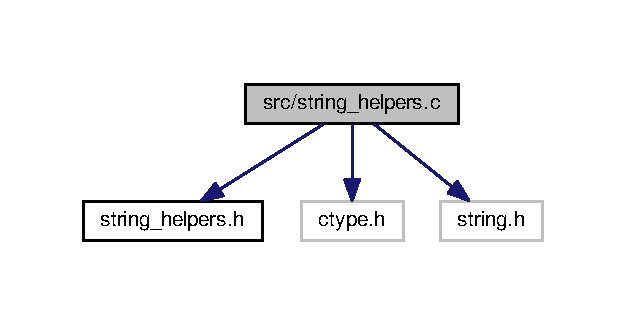
\includegraphics[width=300pt]{string__helpers_8c__incl}
\end{center}
\end{figure}
\subsection*{Functions}
\begin{DoxyCompactItemize}
\item 
int \hyperlink{string__helpers_8c_ad0e6e7f4f903e034b0695058dbefc0a8}{string\-\_\-starts\-With} (char $\ast$line, char $\ast$start)
\item 
int \hyperlink{string__helpers_8c_a6a5539242dc66ee57ed8a30c6bd5979e}{string\-\_\-equals} (char $\ast$str1, char $\ast$str2)
\item 
char $\ast$ \hyperlink{string__helpers_8c_a3ae7aaac50348f5b99fca069b9667bee}{strip\-Out\-Email\-Address} (char $\ast$line)
\item 
int \hyperlink{string__helpers_8c_a20e4e1d1cf8752378fad387f1272fa8d}{string\-\_\-contains} (char $\ast$line, char c)
\item 
int \hyperlink{string__helpers_8c_a358ac995b012642a8d75d63d8f93b122}{valididate\-Email\-Address} (char $\ast$\hyperlink{structemail}{email})
\item 
int \hyperlink{string__helpers_8c_a7b39a32f1f7fdc1f805e61eab1d3f516}{for\-Each\-Character} (char $\ast$input, int($\ast$function)(char input))
\end{DoxyCompactItemize}


\subsection{Function Documentation}
\hypertarget{string__helpers_8c_a7b39a32f1f7fdc1f805e61eab1d3f516}{\index{string\-\_\-helpers.\-c@{string\-\_\-helpers.\-c}!for\-Each\-Character@{for\-Each\-Character}}
\index{for\-Each\-Character@{for\-Each\-Character}!string_helpers.c@{string\-\_\-helpers.\-c}}
\subsubsection[{for\-Each\-Character}]{\setlength{\rightskip}{0pt plus 5cm}int for\-Each\-Character (
\begin{DoxyParamCaption}
\item[{char $\ast$}]{input, }
\item[{int($\ast$)(char input)}]{function}
\end{DoxyParamCaption}
)}}\label{string__helpers_8c_a7b39a32f1f7fdc1f805e61eab1d3f516}
Call a function for each character in a string in case it exits with non-\/zero return that value 
\begin{DoxyParams}{Parameters}
{\em input} & The input string \\
\hline
{\em function} & The function to call for each character \\
\hline
\end{DoxyParams}
\begin{DoxyReturn}{Returns}
Fully depends on function 
\end{DoxyReturn}
\hypertarget{string__helpers_8c_a20e4e1d1cf8752378fad387f1272fa8d}{\index{string\-\_\-helpers.\-c@{string\-\_\-helpers.\-c}!string\-\_\-contains@{string\-\_\-contains}}
\index{string\-\_\-contains@{string\-\_\-contains}!string_helpers.c@{string\-\_\-helpers.\-c}}
\subsubsection[{string\-\_\-contains}]{\setlength{\rightskip}{0pt plus 5cm}int string\-\_\-contains (
\begin{DoxyParamCaption}
\item[{char $\ast$}]{line, }
\item[{char}]{c}
\end{DoxyParamCaption}
)}}\label{string__helpers_8c_a20e4e1d1cf8752378fad387f1272fa8d}
Return if line contains c 
\begin{DoxyParams}{Parameters}
{\em line} & String to check for a certain character \\
\hline
{\em c} & the character to check for \\
\hline
\end{DoxyParams}
\begin{DoxyReturn}{Returns}
1 if line does contain c 
\end{DoxyReturn}
\hypertarget{string__helpers_8c_a6a5539242dc66ee57ed8a30c6bd5979e}{\index{string\-\_\-helpers.\-c@{string\-\_\-helpers.\-c}!string\-\_\-equals@{string\-\_\-equals}}
\index{string\-\_\-equals@{string\-\_\-equals}!string_helpers.c@{string\-\_\-helpers.\-c}}
\subsubsection[{string\-\_\-equals}]{\setlength{\rightskip}{0pt plus 5cm}int string\-\_\-equals (
\begin{DoxyParamCaption}
\item[{char $\ast$}]{str1, }
\item[{char $\ast$}]{str2}
\end{DoxyParamCaption}
)}}\label{string__helpers_8c_a6a5539242dc66ee57ed8a30c6bd5979e}
Simple check if str1 is equal to str2 
\begin{DoxyParams}{Parameters}
{\em str1} & Input string 1 \\
\hline
{\em str2} & Input string 2 \\
\hline
\end{DoxyParams}
\begin{DoxyReturn}{Returns}
It'll return 1 in case they're equal, else it'll return 0 
\end{DoxyReturn}
\hypertarget{string__helpers_8c_ad0e6e7f4f903e034b0695058dbefc0a8}{\index{string\-\_\-helpers.\-c@{string\-\_\-helpers.\-c}!string\-\_\-starts\-With@{string\-\_\-starts\-With}}
\index{string\-\_\-starts\-With@{string\-\_\-starts\-With}!string_helpers.c@{string\-\_\-helpers.\-c}}
\subsubsection[{string\-\_\-starts\-With}]{\setlength{\rightskip}{0pt plus 5cm}int string\-\_\-starts\-With (
\begin{DoxyParamCaption}
\item[{char $\ast$}]{str1, }
\item[{char $\ast$}]{str2}
\end{DoxyParamCaption}
)}}\label{string__helpers_8c_ad0e6e7f4f903e034b0695058dbefc0a8}
Simple check if str1 starts with str2 
\begin{DoxyParams}{Parameters}
{\em str1} & Input string \\
\hline
{\em str2} & String line has to start with \\
\hline
\end{DoxyParams}
\begin{DoxyReturn}{Returns}
It'll return 1 in case line does start with start, else it'll return 0 
\end{DoxyReturn}
\hypertarget{string__helpers_8c_a3ae7aaac50348f5b99fca069b9667bee}{\index{string\-\_\-helpers.\-c@{string\-\_\-helpers.\-c}!strip\-Out\-Email\-Address@{strip\-Out\-Email\-Address}}
\index{strip\-Out\-Email\-Address@{strip\-Out\-Email\-Address}!string_helpers.c@{string\-\_\-helpers.\-c}}
\subsubsection[{strip\-Out\-Email\-Address}]{\setlength{\rightskip}{0pt plus 5cm}char$\ast$ strip\-Out\-Email\-Address (
\begin{DoxyParamCaption}
\item[{char $\ast$}]{line}
\end{DoxyParamCaption}
)}}\label{string__helpers_8c_a3ae7aaac50348f5b99fca069b9667bee}
Return just the email address 
\begin{DoxyParams}{Parameters}
{\em line} & Raw line from the S\-M\-T\-P client \\
\hline
\end{DoxyParams}
\begin{DoxyReturn}{Returns}
A new string with just the email address 
\end{DoxyReturn}
\begin{DoxyNote}{Note}
line is not freed. 
\end{DoxyNote}
\hypertarget{string__helpers_8c_a358ac995b012642a8d75d63d8f93b122}{\index{string\-\_\-helpers.\-c@{string\-\_\-helpers.\-c}!valididate\-Email\-Address@{valididate\-Email\-Address}}
\index{valididate\-Email\-Address@{valididate\-Email\-Address}!string_helpers.c@{string\-\_\-helpers.\-c}}
\subsubsection[{valididate\-Email\-Address}]{\setlength{\rightskip}{0pt plus 5cm}int valididate\-Email\-Address (
\begin{DoxyParamCaption}
\item[{char $\ast$}]{email}
\end{DoxyParamCaption}
)}}\label{string__helpers_8c_a358ac995b012642a8d75d63d8f93b122}
Check if this emailaddress contains 1 at sign and is only made up of letters and/or numbers 
\begin{DoxyParams}{Parameters}
{\em email} & The email address to check \\
\hline
\end{DoxyParams}
\begin{DoxyReturn}{Returns}
1 if it's valid 
\end{DoxyReturn}

\addcontentsline{toc}{part}{Index}
\printindex
\end{document}
